% !TeX spellcheck = en_US
%%
%% Text of diploma thesis
%%
%% Tomáš Zítka
%%

%needed packages
\documentclass{book}
\usepackage[english]{babel} 
\usepackage{a4wide}
\usepackage{graphicx}
\usepackage[utf8]{inputenc}
\usepackage{enumerate}
\usepackage{amssymb, amsmath}
\usepackage{natbib}
\usepackage{ae}

\usepackage[all]{xy}







% colors
\usepackage[usenames,dvipsnames]{xcolor}
\definecolor{deepblue}{rgb}{0, 0, 0.5}
\definecolor{deepred}{rgb}{0.6, 0, 0}
\definecolor{deepgreen}{rgb}{0, 0.5, 0}


\usepackage{tikz}

% links style
\usepackage[unicode]{hyperref}
\hypersetup{
	colorlinks,
	linkcolor={red!50!black},
	citecolor={blue!50!black},
	urlcolor={blue!80!black}
}


% acronyms
%\usepackage[acronym, xindy]{glossaries}
%\makenoidxglossaries
%\input{./texts/zkratky}

% code typeseting
\usepackage{listings}
\lstset{numbers=none,
		stepnumber=2,
		numbersep=5pt,
		numbers=none,
		tabsize=4,	
		frame=lines,
		language=Python,
		otherkeywords={self},
		breaklines=true,
		breakatwhitespace=true,
		basicstyle=\ttfamily,%\footnotesize
		keywordstyle=\bfseries\color{deepblue},
		commentstyle=\small\color{gray},
		stringstyle=\color{deepgreen},
		showstringspaces=false
}


%inline code typesseting
\newcommand{\shellcmd}[1]{\texttt{#1}}
\newcommand{\pysauce}[1]{\lstinline!#1!}

% some logos 
\providecommand{\Microsoft}{{\sffamily Microsoft}}	
\providecommand{\Windows}{{\sffamily Windows}}	

%TO-DOcomand
\providecommand{\todo}{\textbf{TODO }}


% math stuff
\newtheorem{theorem}{Theorem}
\newtheorem{definition}{Definition}
\newtheorem{princ}{Principle}
\newtheorem{axiom}{Axiom}[chapter]
\newtheorem{claim}{Proposition}
\newtheorem{Lemma}{Lemma}

\providecommand{\bracesanddots}[4]{$\langle$#1$\rangle$:$\langle$#2$\rangle$:$\langle$#3$\rangle$:$\langle$#4$\rangle$}
\providecommand{\anglebracs}[1]{$\langle$#1$\rangle$}
\providecommand{\manglebracs}[1]{\langle#1\rangle}
\providecommand{\norm}[1]{\left\lVert#1\right\rVert}
\providecommand{\abs}[1]{\left\lvert#1\right\rvert}
\providecommand{\doteq}{\,\dot = \,}
\newcommand{\pdiff}[2]{\frac{\partial#1}{\partial#2}}
\newcommand{\fdiff}[2]{\frac{\text{d}#1}{\text{d}#2}}
\newcommand{\Laplace}{\Delta}
\newcommand{\DAlambert}{\mathop{}\!\mathbin\Box}

% number classes
\providecommand{\realc}{\mathbb{R}}
\providecommand{\naturc}{\mathbb{N}}
\providecommand{\finaturc}{\mathbb{FN}}
\providecommand{\fisnaturc}{\mathbb{F^*N}}
\providecommand{\comc}{\mathbb{C}}

% classes
\providecommand{\bV}{\mathbf{V}}
\providecommand{\bFV}{\mathbf{FV}}
\providecommand{\bFsV}{\mathbf{F^*V}}

% domains
\providecommand{\fU}{\mathfrak{U}}
\providecommand{\fM}{\mathfrak{M}}

% universes
\providecommand{\cala}{\mathcal{A}}
\providecommand{\calc}{\mathcal{C}}
\providecommand{\calv}{\mathcal{V}}
\providecommand{\calw}{\mathcal{W}}

% convenient math functions
\newcommand\tg{\qopname\relax o{tg}}
\newcommand\tgh{\qopname\relax o{tgh}}
\newcommand\sign{\qopname\relax o{sign}}
\newcommand\cotg{\qopname\relax o{cotg}}
\newcommand\atg{\qopname\relax o{arctg}}
\newcommand\im{\qopname\relax o{Im}}
\newcommand\re{\qopname\relax o{Re}}

\newcommand{\Cls}{\mathrm{Cls}}
\newcommand{\Set}{\mathrm{Set}}
\newcommand{\Fin}{\mathrm{Fin}}
\newcommand{\Nat}{\mathrm{Nat}}

\newcommand{\dom}{\mathrm{dom}}
\newcommand{\rng}{\mathrm{rng}}

% terms
\newcommand{\st}{$\sigma$-tříd}
\newcommand{\pt}{$\pi$-tříd}


\numberwithin{equation}{section}
\usepackage{chngcntr}
\counterwithout{figure}{chapter}
\numberwithin{table}{section}


\begin{document}

\tableofcontents

\newpage
\section{Diffusion \& advection}
\begin{example}[Advection-diffusion 2D]
\label{ex:quart1}
Based on Example 1 from \cite{Antonietti2013},
we will solve equation \eqref{eq:ex_advdiff} in $\Omega = \langle 0, 1 \rangle^2$.
%\begin{equation}
%	\pdiff{u}{x} + \pdiff{u}{y} - D \cdot \left( \pdiff{^2 u}{x^2} + \pdiff{^2 
%u}{y^2} \right) = g
%\end{equation}
%i.e
%\begin{equation}
%	\vec{a} \cdot \nabla u - D \Delta u = g
%\end{equation}
%where $\vec{a} = [1, 1]^T$ is advection velocity, $D$ is diffusion coefficient 
%and $g$ is a source function.
We setup boundary conditions and source function $g$ in such way that 
the exact solution $u_{exact}$ is
\begin{equation}
	u_{exact}(x,y) =  -{\left(y^{2} - y\right)} \sin\left(2 \, \pi x\right).
\end{equation}
Solving for $g$ yields
\begin{equation}
	g = \\
	 -2 \, \pi {\left(y^{2} - y\right)} \cos\left(2 \, \pi x\right) - 2 \, {\left(2 \, 
	 \pi^{2} 
	{\left(y^{2} - y\right)} \sin\left(2 \, \pi x\right) - D\sin\left(2 \, \pi 
	x\right)\right)} 
	 - {\left(2 \, y - 1\right)} \sin\left(2 \, \pi x\right).
\end{equation}
matching  boundary conditions are
\begin{equation}
	\begin{aligned}
	&u(x) = 0, \quad x \in \partial\Omega\\
	&\nabla u(x) = [-2\pi(y^2 - y)\cos(2 \pi x), -(2 y - 1)\sin(2\pi  x)]^T, \quad x \in 
	\partial\Omega.
	\end{aligned}
\end{equation}
Different values of coefficient $C_w$ in penalty term then yield different 
convergence behavior as demonstrated in Figure \ref{fig:qconv1} and 
\Cref{fig:orders_quarteroni1}. Both figures illustrate "gluing" effect of penalty term 
which increases with $C_w$ coefficient and counteracts discontinuities between elements 
which are the main source of error in this example.

\begin{figure}[h!]
	\centering
	\begin{tabular}{p{0.5\textwidth} p{0.5\textwidth}}
		\vspace{0pt} 
		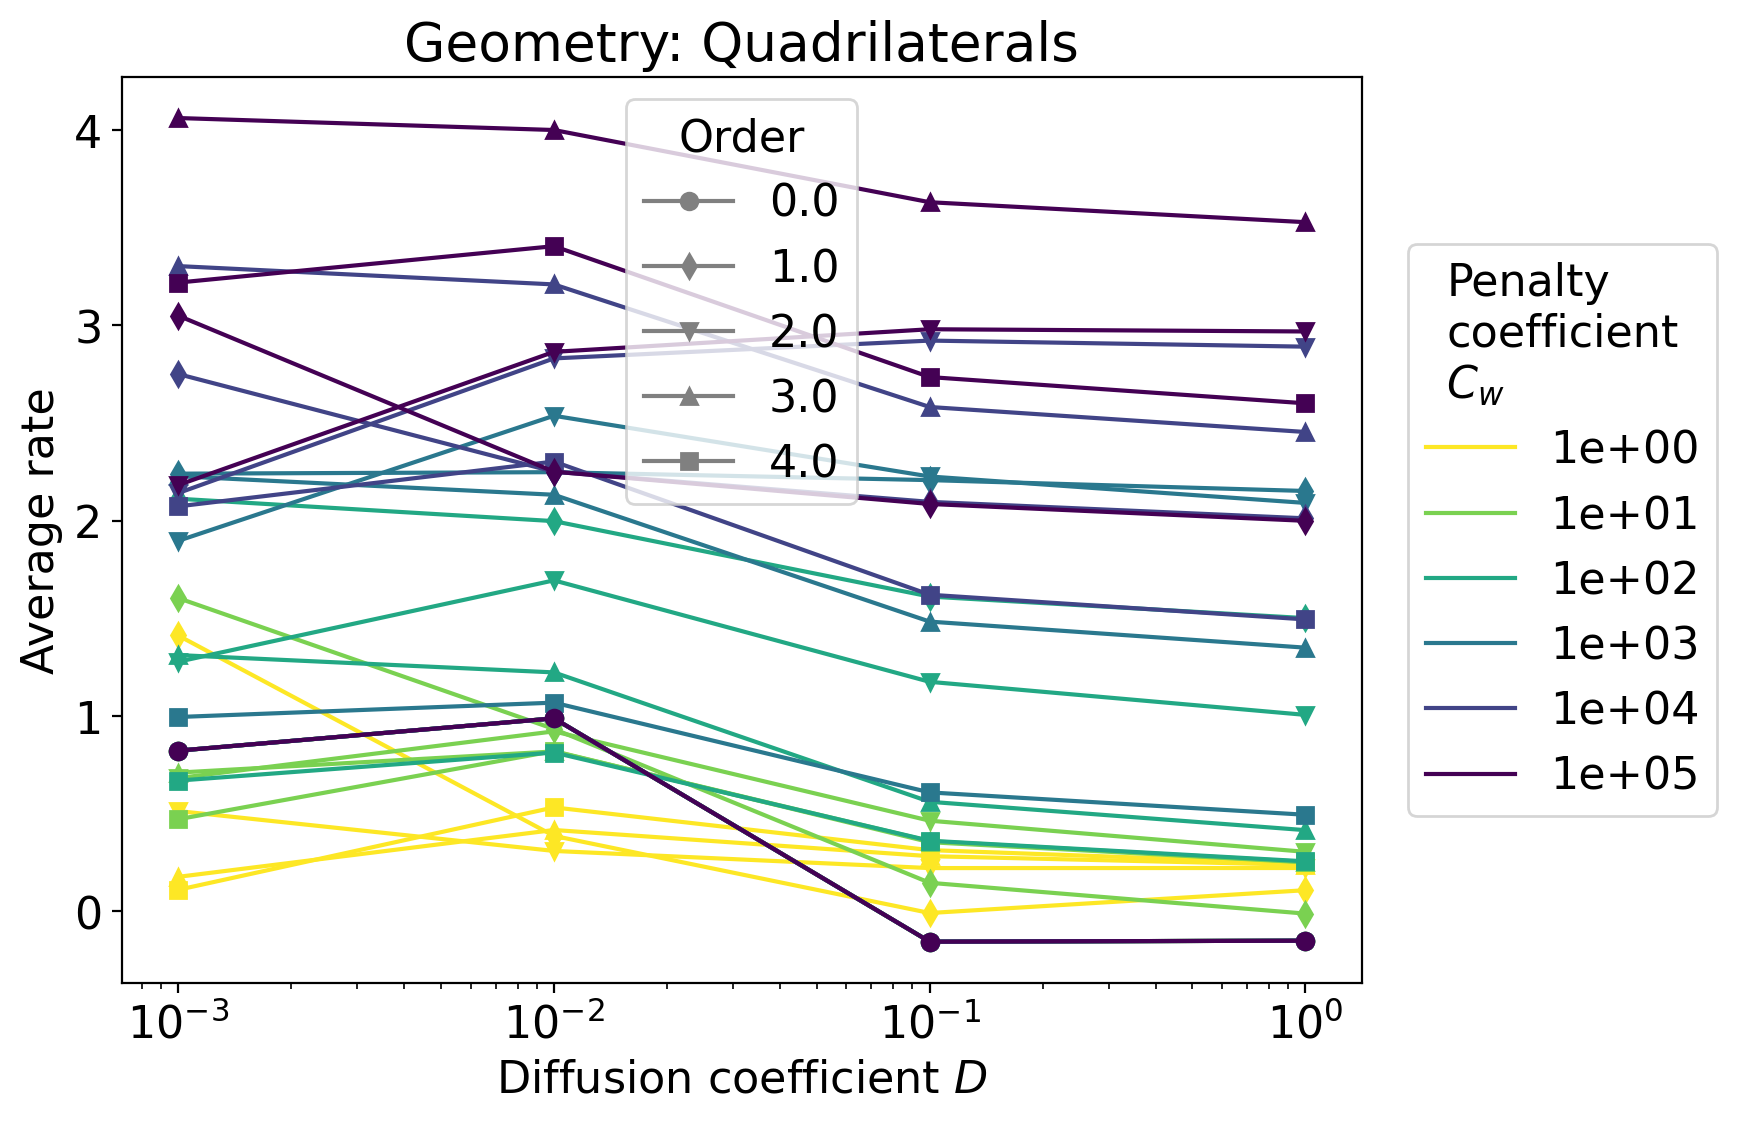
\includegraphics[width=0.49\textwidth]{../figs/parametric/advdiff_2D/ord_quarteroni1_2_4}
		&
		\vspace{0pt} 
		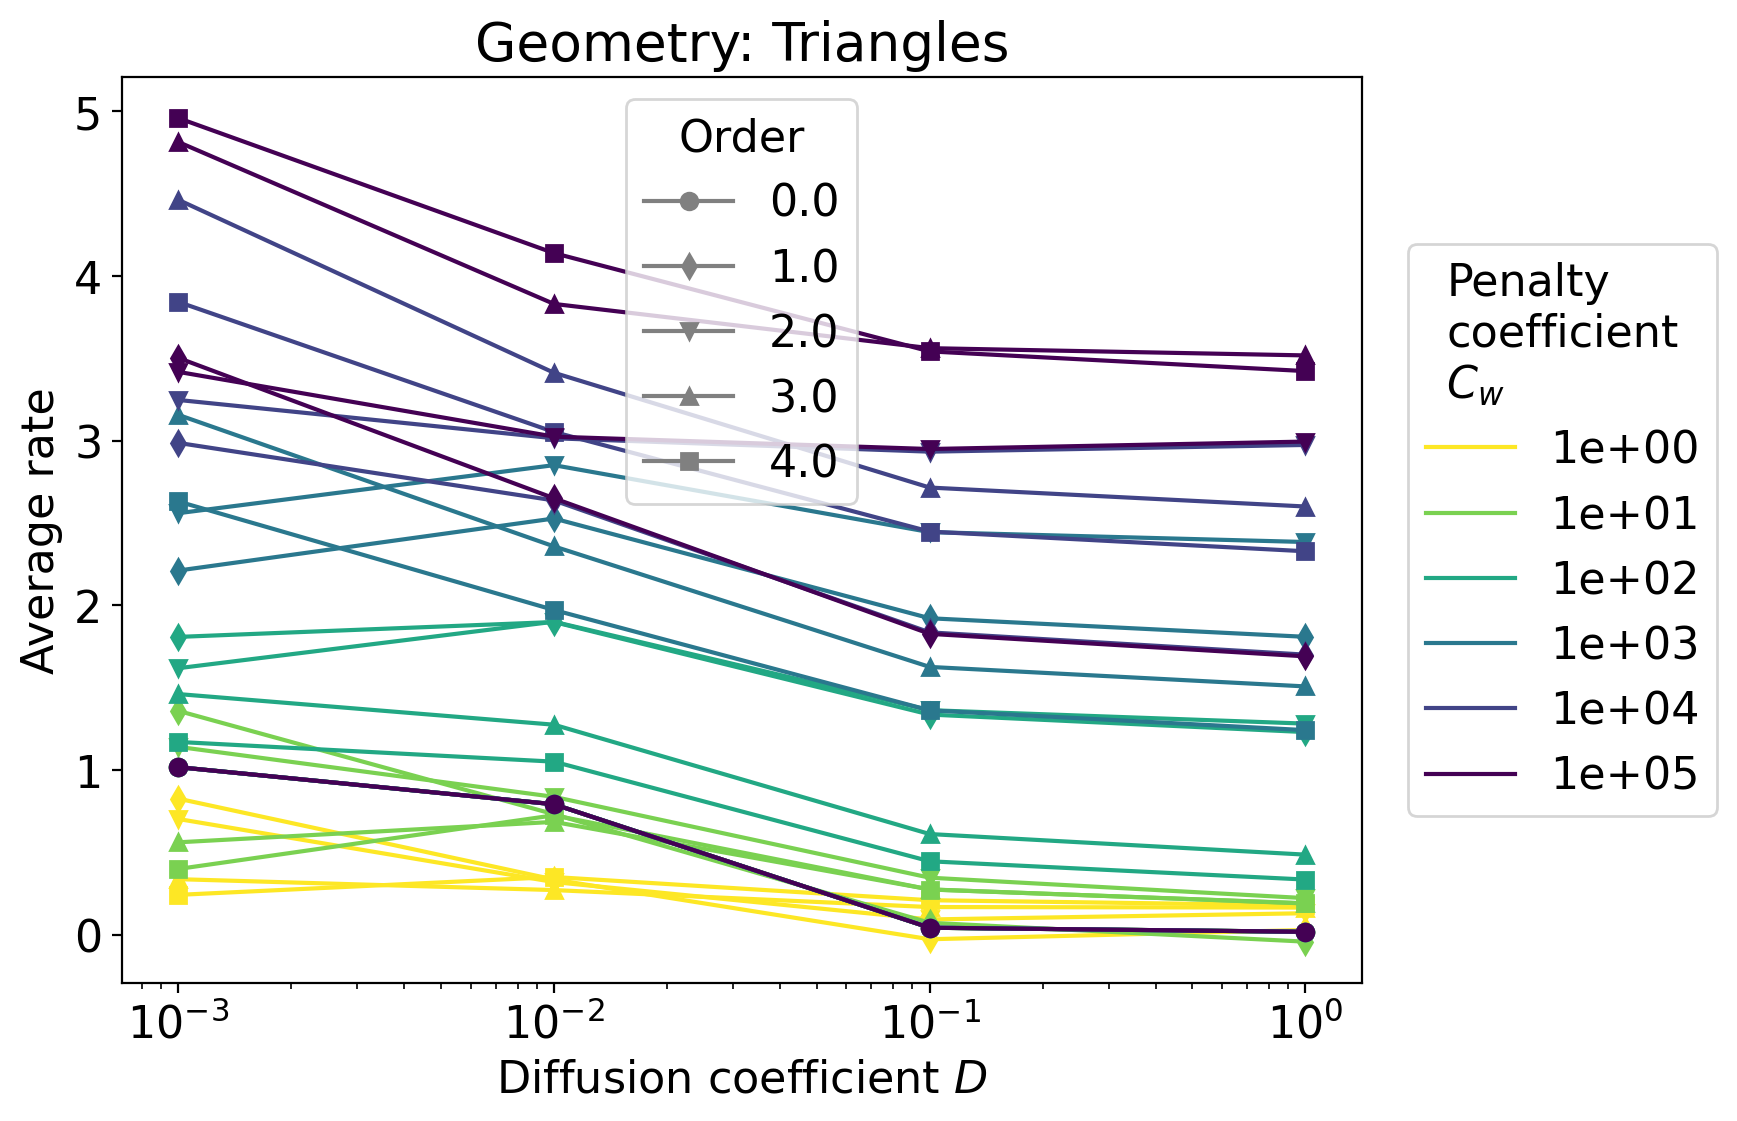
\includegraphics[width=0.49\textwidth]{../figs/parametric/advdiff_2D/ord_quarteroni1_2_3}
	\end{tabular}
	
%	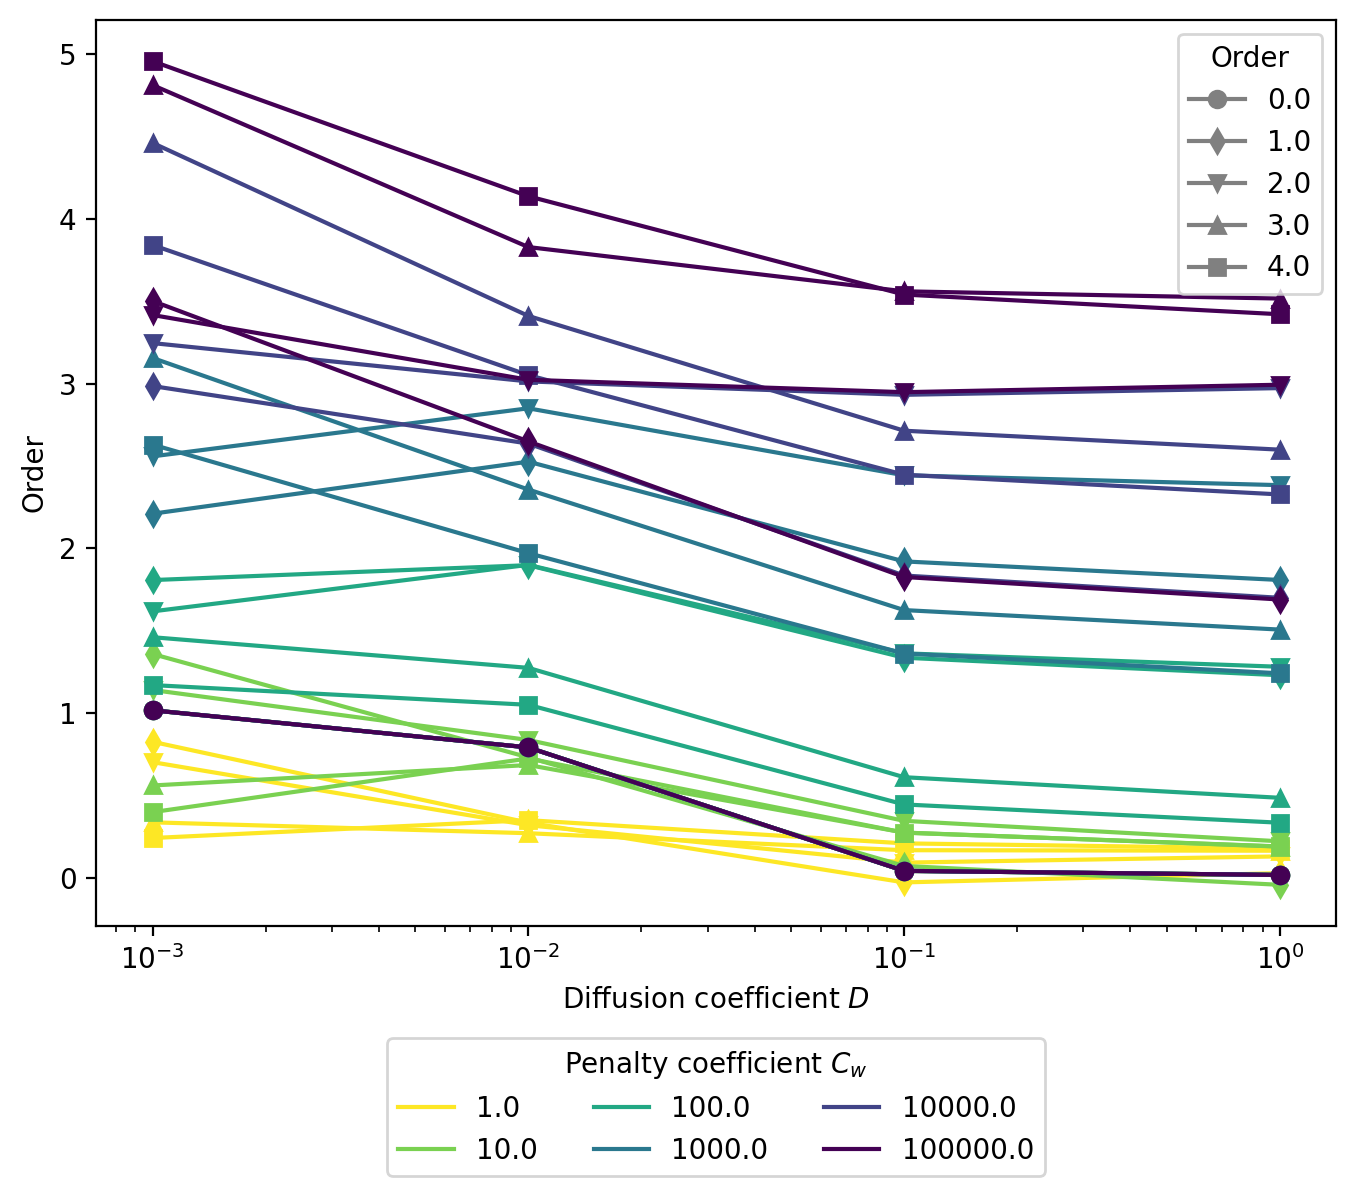
\includegraphics[scale=.5]{../figs/parametric/advdiff_2D/ord_quarteroni1}
	\caption{\Cref{ex:quart1} average order for different choice of $C_w$}
	\label{fig:orders_quarteroni1}
\end{figure}



\end{example}
\begin{figure}[p!]
	\centering
	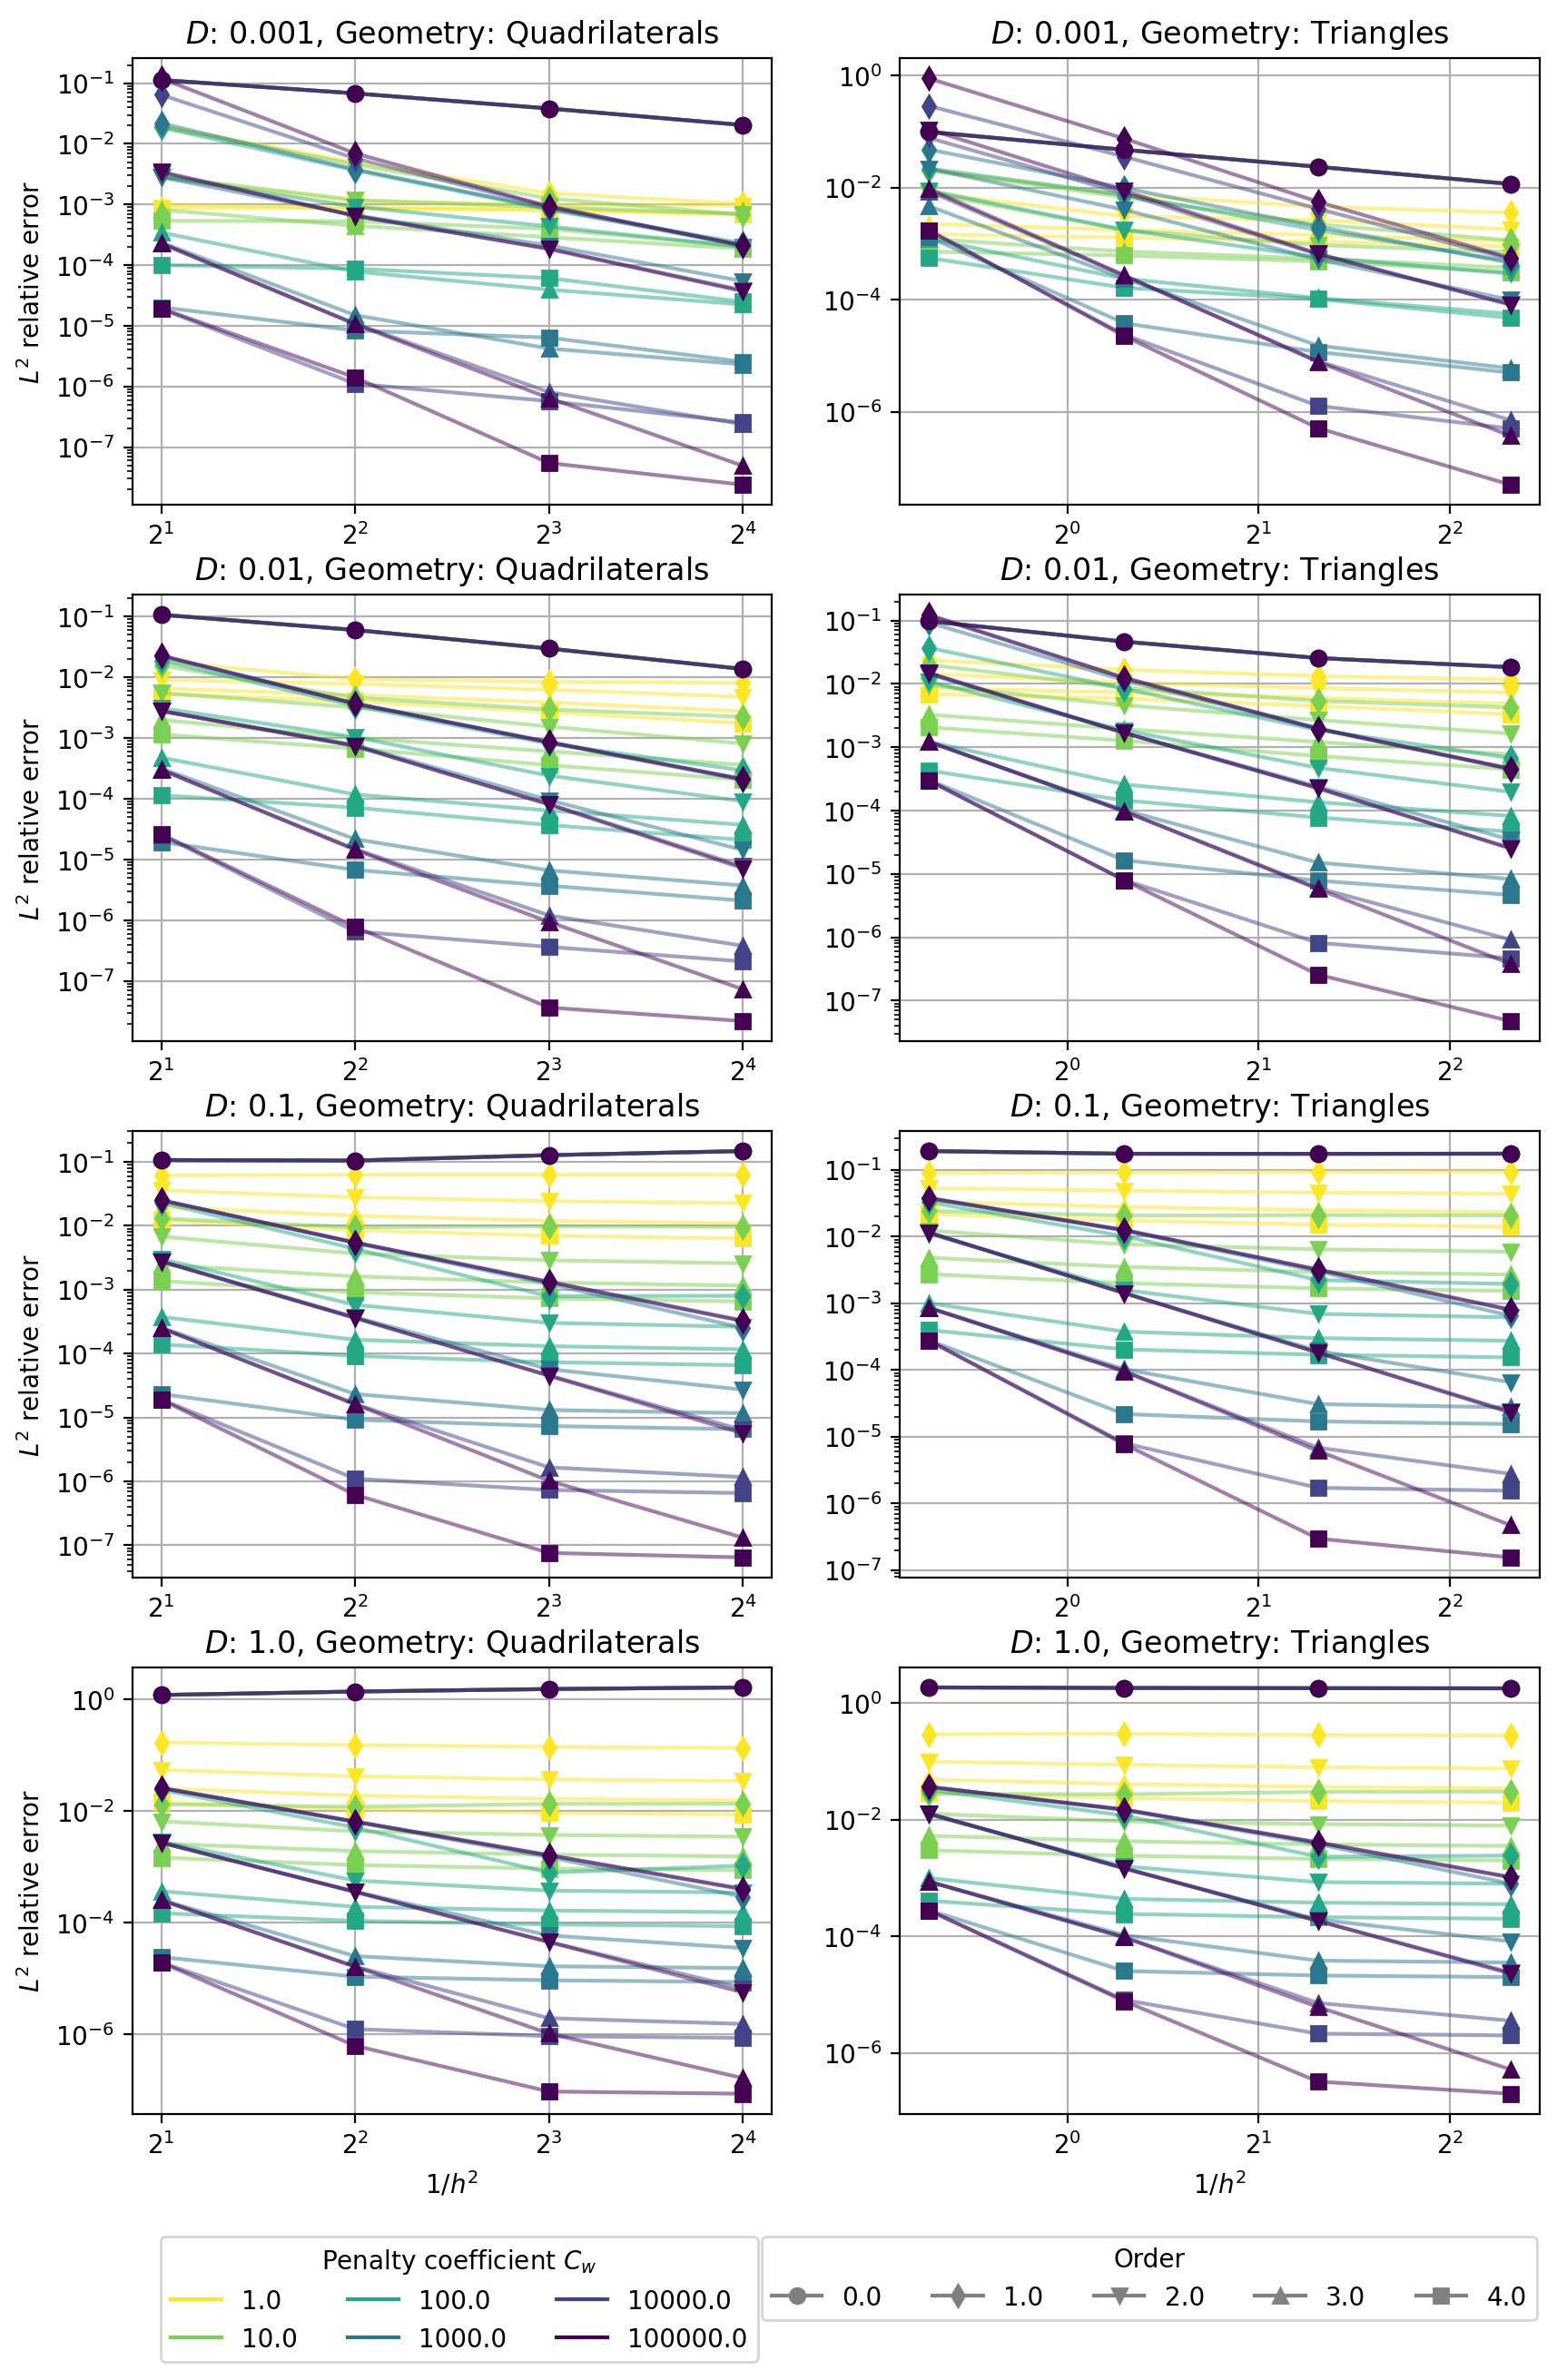
\includegraphics[height=\textheight]{../figs/parametric/advdiff_2D/quarteroni1}
	\caption{\Cref{ex:quart1} convergence graphs for different choice of $C_w$}
	\label{fig:qconv1}
\end{figure}

\newpage
\begin{example}[Advection-diffusion 2D]
\label{ex:quart2}
Based on Example 2 \cite{Antonietti2013},
in $\Omega = \langle 0, 1 \rangle^2$ we will again solve equation \eqref{eq:ex_advdiff}
%\begin{equation}
%	\pdiff{u}{x} + \pdiff{u}{y} - D \cdot \left( \pdiff{^2 u}{x^2} + \pdiff{^2 
%	u}{y^2} \right) = g
%\end{equation}
%i.e
%\begin{equation}
%	\vec{a} \cdot \nabla u - D \Delta u = g
%\end{equation}
%where $\vec{a} = [1, 1]^T$ is advection velocity and $D$ is diffusion 
%coefficient and $g$ is a source function. 
We setup boundary condition and source function in such way that the exact 
solution $u_{exact}$ is
\begin{equation}
	u_{exact} =  -\arctan\left(\frac{4 \, {\left(2 \, x - 1\right)}^{2} + 4 \, {\left(2 
	\, y - 1\right)}^{2} - 
	1}{16 \, \sqrt{\mathit{D}}}\right).
\end{equation}
We omit analytical forms of $g$ and boundary conditions for brevity, they can be found in 
the code.
Different values of coefficient $C_w$ in penalty term yield different 
convergence behavior as demonstrated in Figure \ref{fig:conv_qart2} and 
\Cref{fig:orders_quarteroni2}.
\end{example}

\begin{figure}[h!]
\centering
\begin{tabular}{p{0.5\textwidth} p{0.5\textwidth}}
	\vspace{0pt} 
	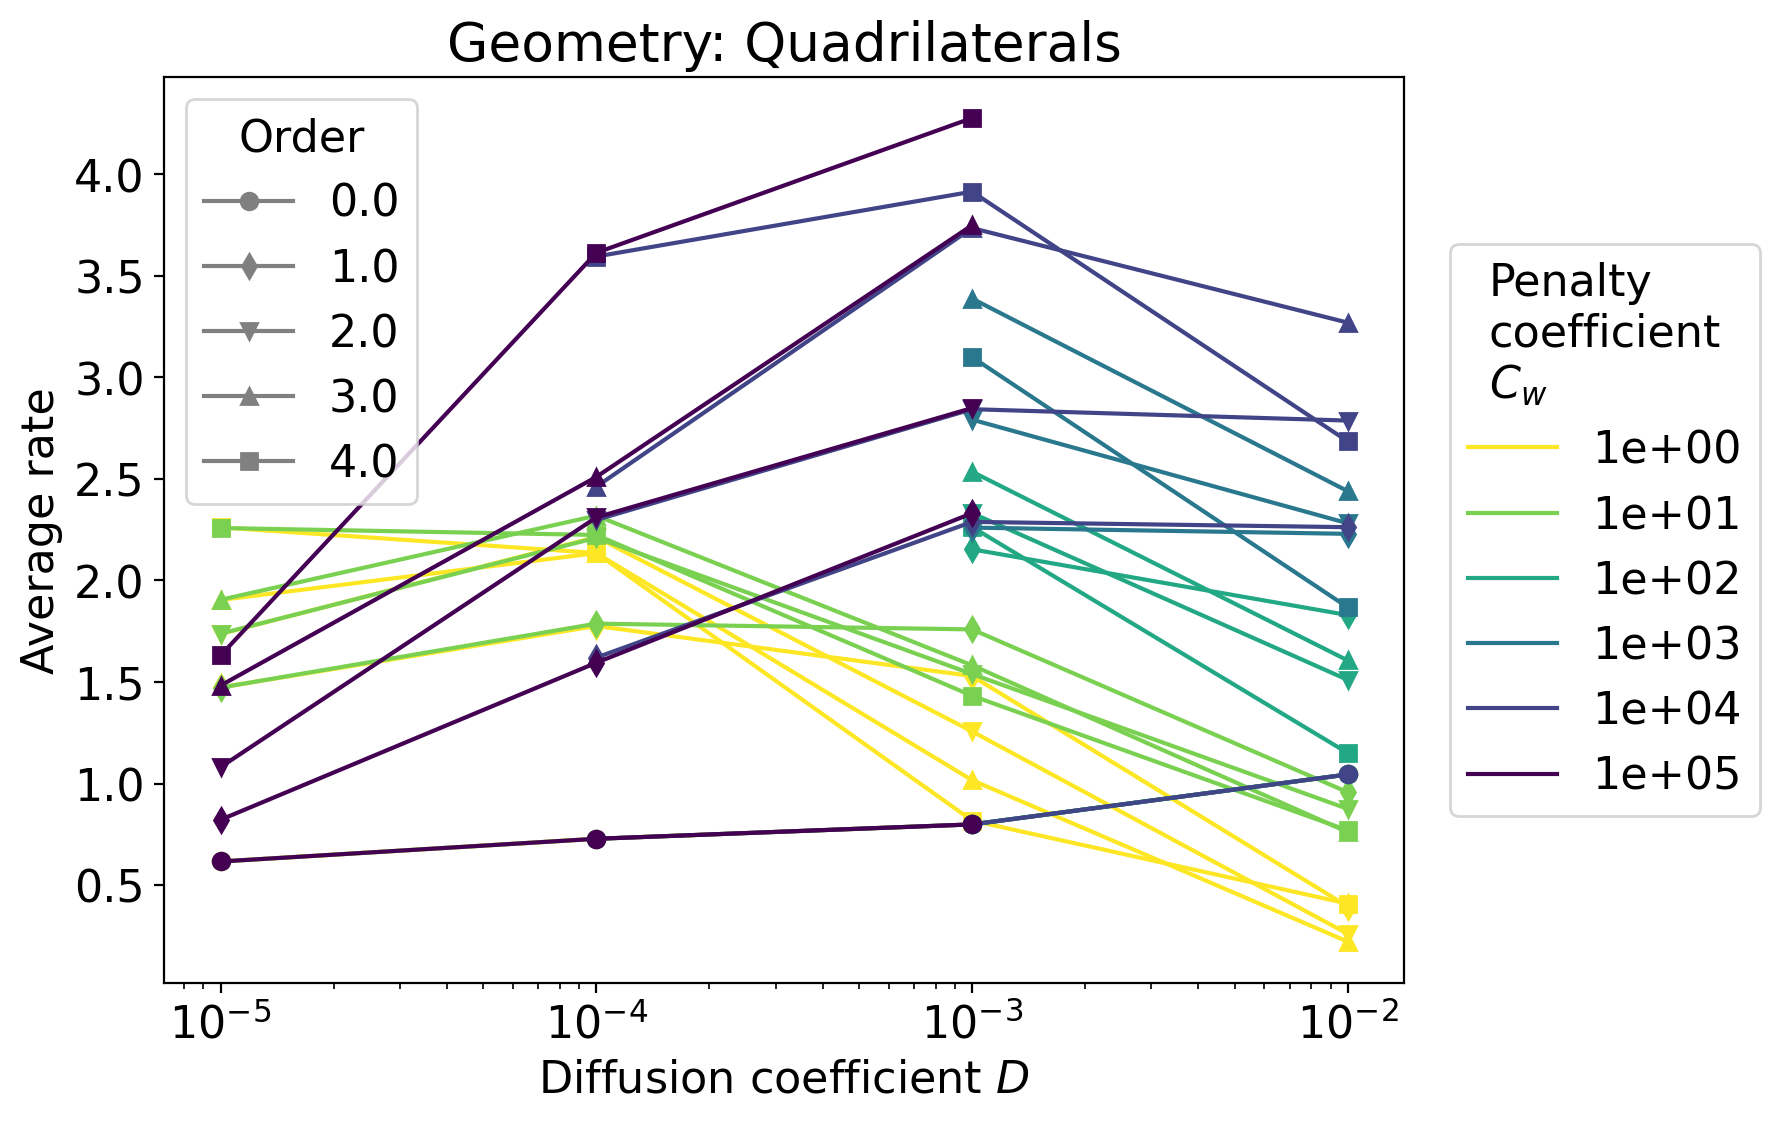
\includegraphics[width=0.49\textwidth]{../figs/parametric/advdiff_2D/ord_quarteroni2_2_4}
	&
	\vspace{0pt} 
	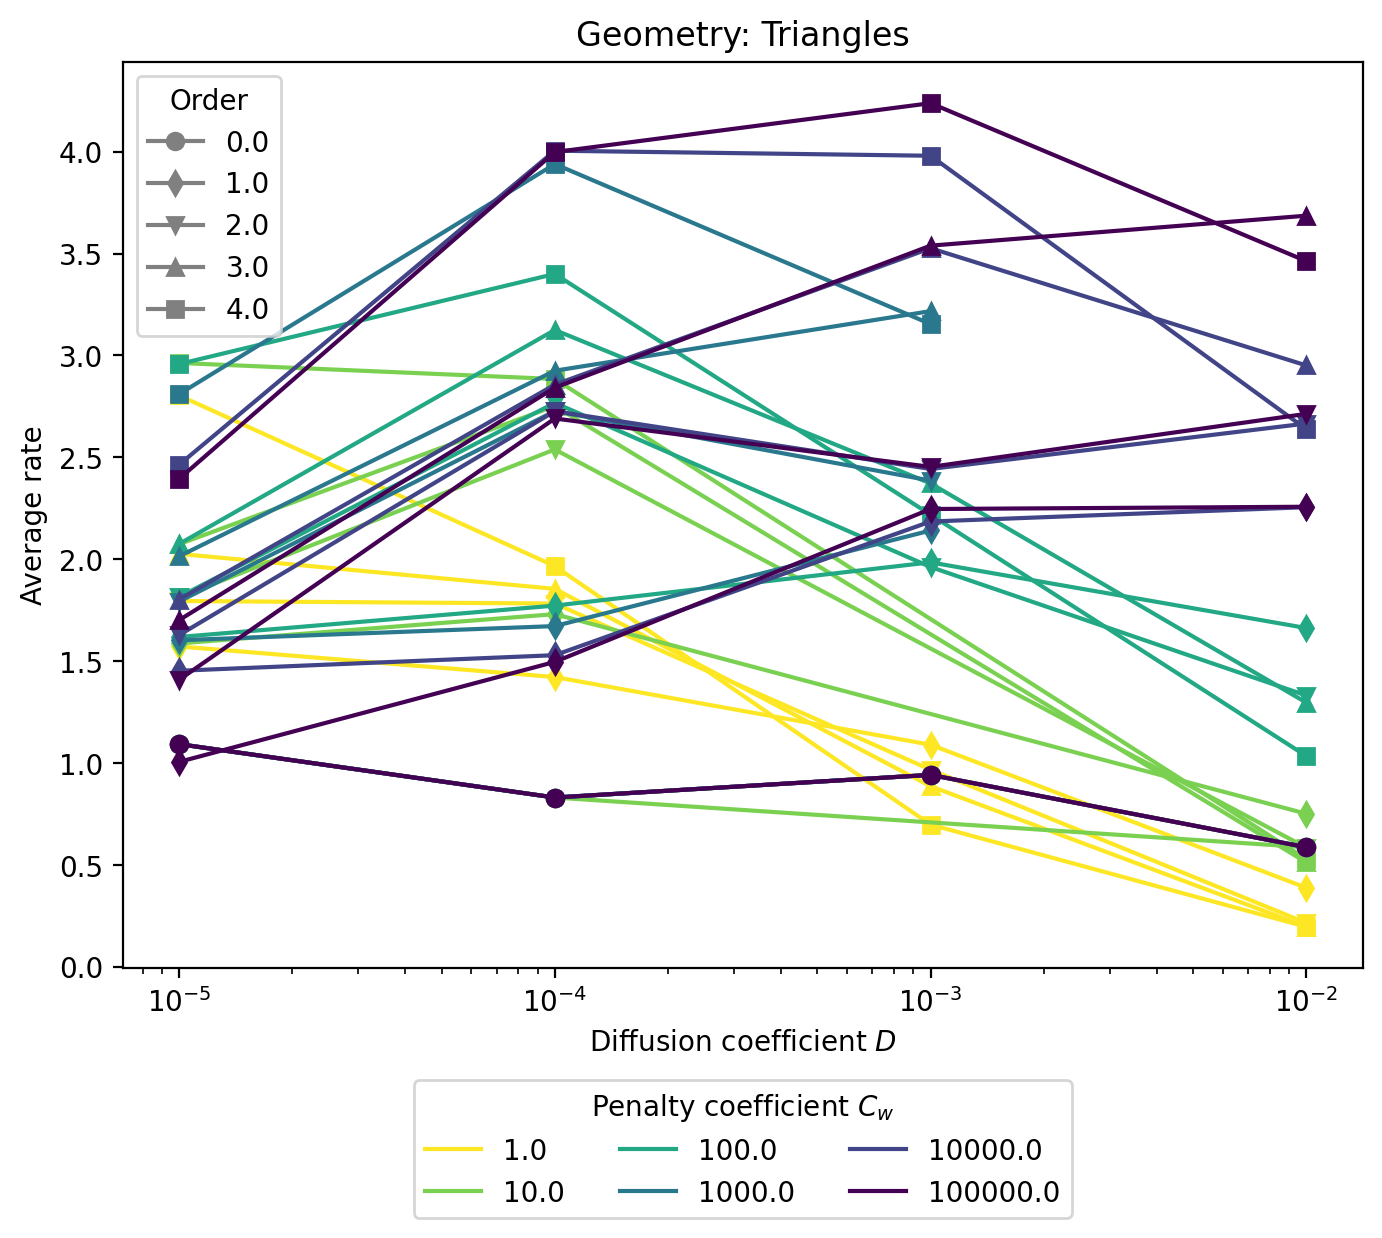
\includegraphics[width=0.49\textwidth]{../figs/parametric/advdiff_2D/ord_quarteroni2_2_3}
\end{tabular}
\caption{\Cref{ex:quart2} average order for different choice of $C_w$}
\label{fig:orders_quarteroni2}
\end{figure}


\begin{figure}[p!]
	\centering
	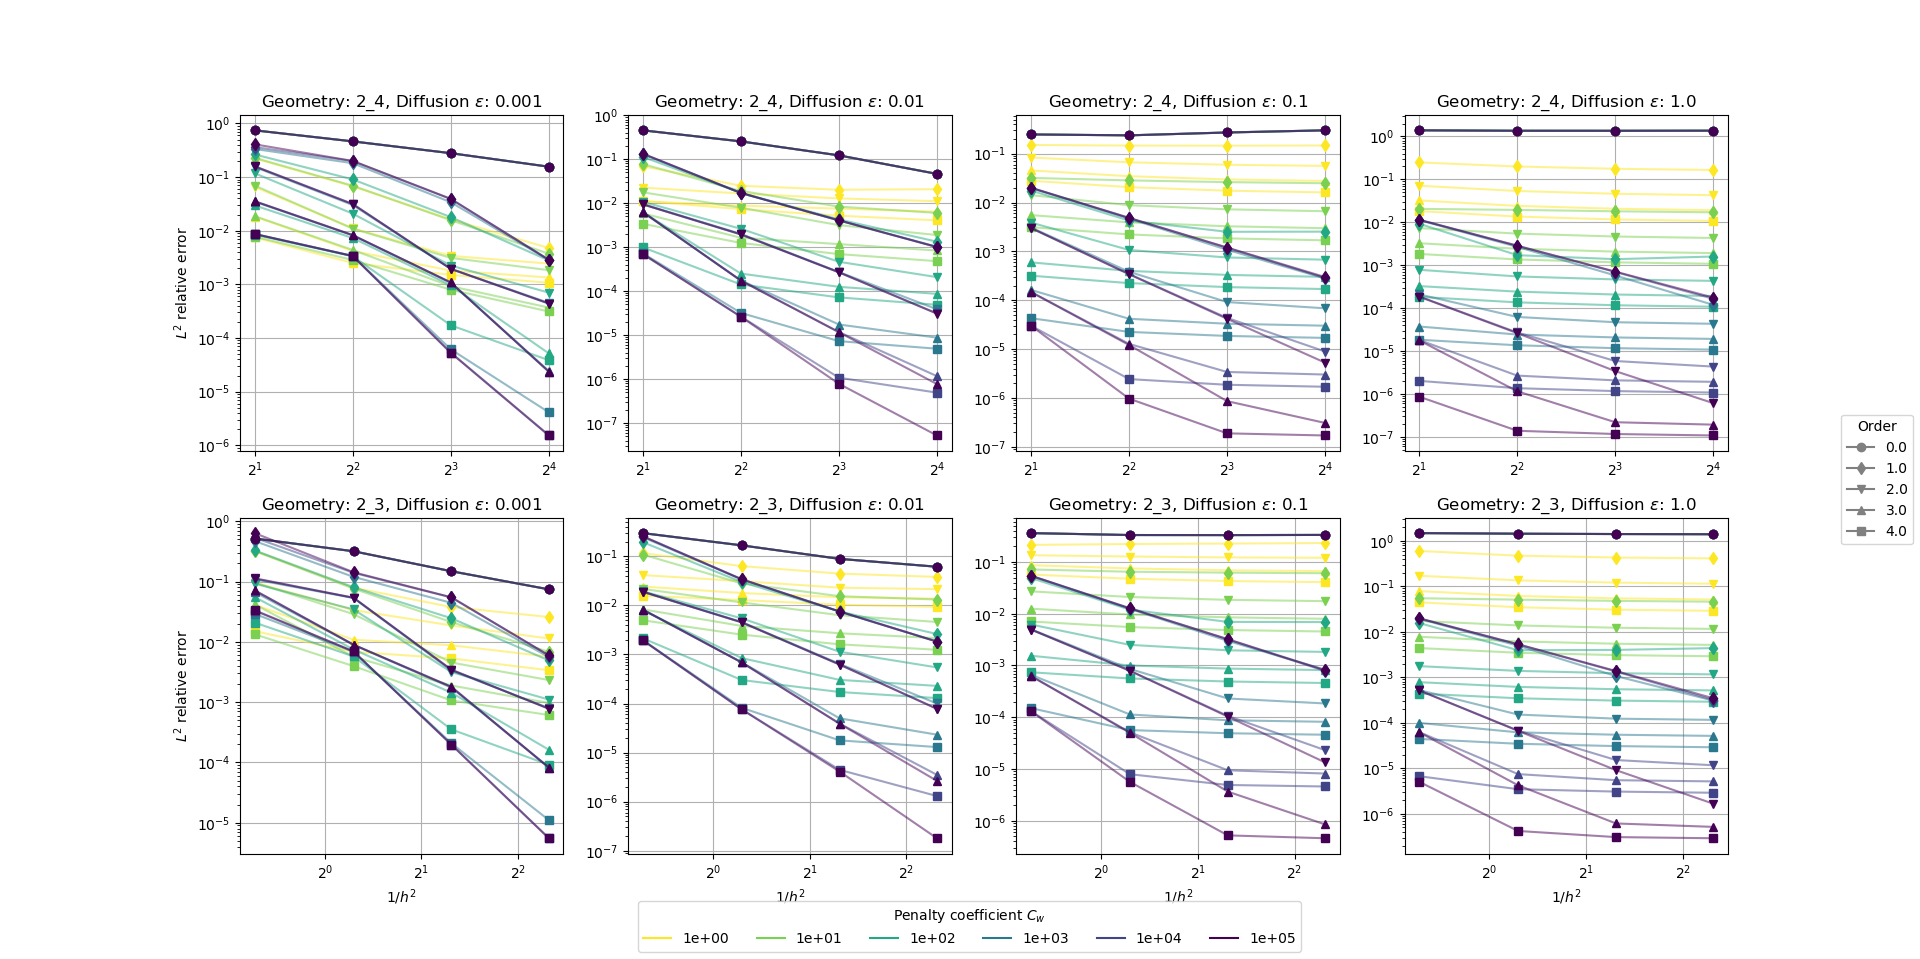
\includegraphics[height=\textheight]{../figs/parametric/advdiff_2D/quarteroni2.png}
	
	\caption{\Cref{ex:quart2} convergence graphs for different choice of $C_w$}
	\label{fig:conv_qart2}
\end{figure}

\newpage
\begin{example}[Advection-diffusion 2D]
\label{ex:quart3}
Based on Example 3 in \cite{Antonietti2013},
in $\Omega = \langle 0, 1 \rangle^2$ we will once again solve equation
%\begin{equation}
%	\pdiff{u}{x} + \pdiff{u}{y} - D \cdot \left( \pdiff{^2 u}{x^2} + \pdiff{^2 
%	u}{y^2} \right) = g
%\end{equation}
%i.e
%\begin{equation}
%	\vec{a} \cdot \nabla u - D \Delta u = g
%\end{equation}
%where $\vec{a} = [1, 1]^T$ is advection velocity and $D$ is diffusion 
%coefficient and $g$ is a source function.
We set up boundary condition and source function in such a way that the exact 
solution $u_{exact}$ is
\begin{equation}
	u_{exact} = -xy + x +y + \frac{\exp{\left(-\frac{{\left(x - 1\right)} {\left(y - 
	1\right)}}{D}\right)} - 
	\exp{\left(-\frac{1}{D}\right)}}{\exp{\left(-\frac{1}{D}\right)} 
	- 1}.
\end{equation}
We omit analytical forms of $g$ and boundary conditions for brevity, they can found in 
the code. Different values of 
coefficient $C_w$ in penalty term yield different convergence behavior as 
demonstrated in Figure 
\ref{fig:conv_qart3} and \Cref{fig:orders_quarteroni3}
\end{example}

\begin{figure}[h!]
	\centering
	\begin{tabular}{p{0.5\textwidth} p{0.5\textwidth}}
	\vspace{0pt} 
	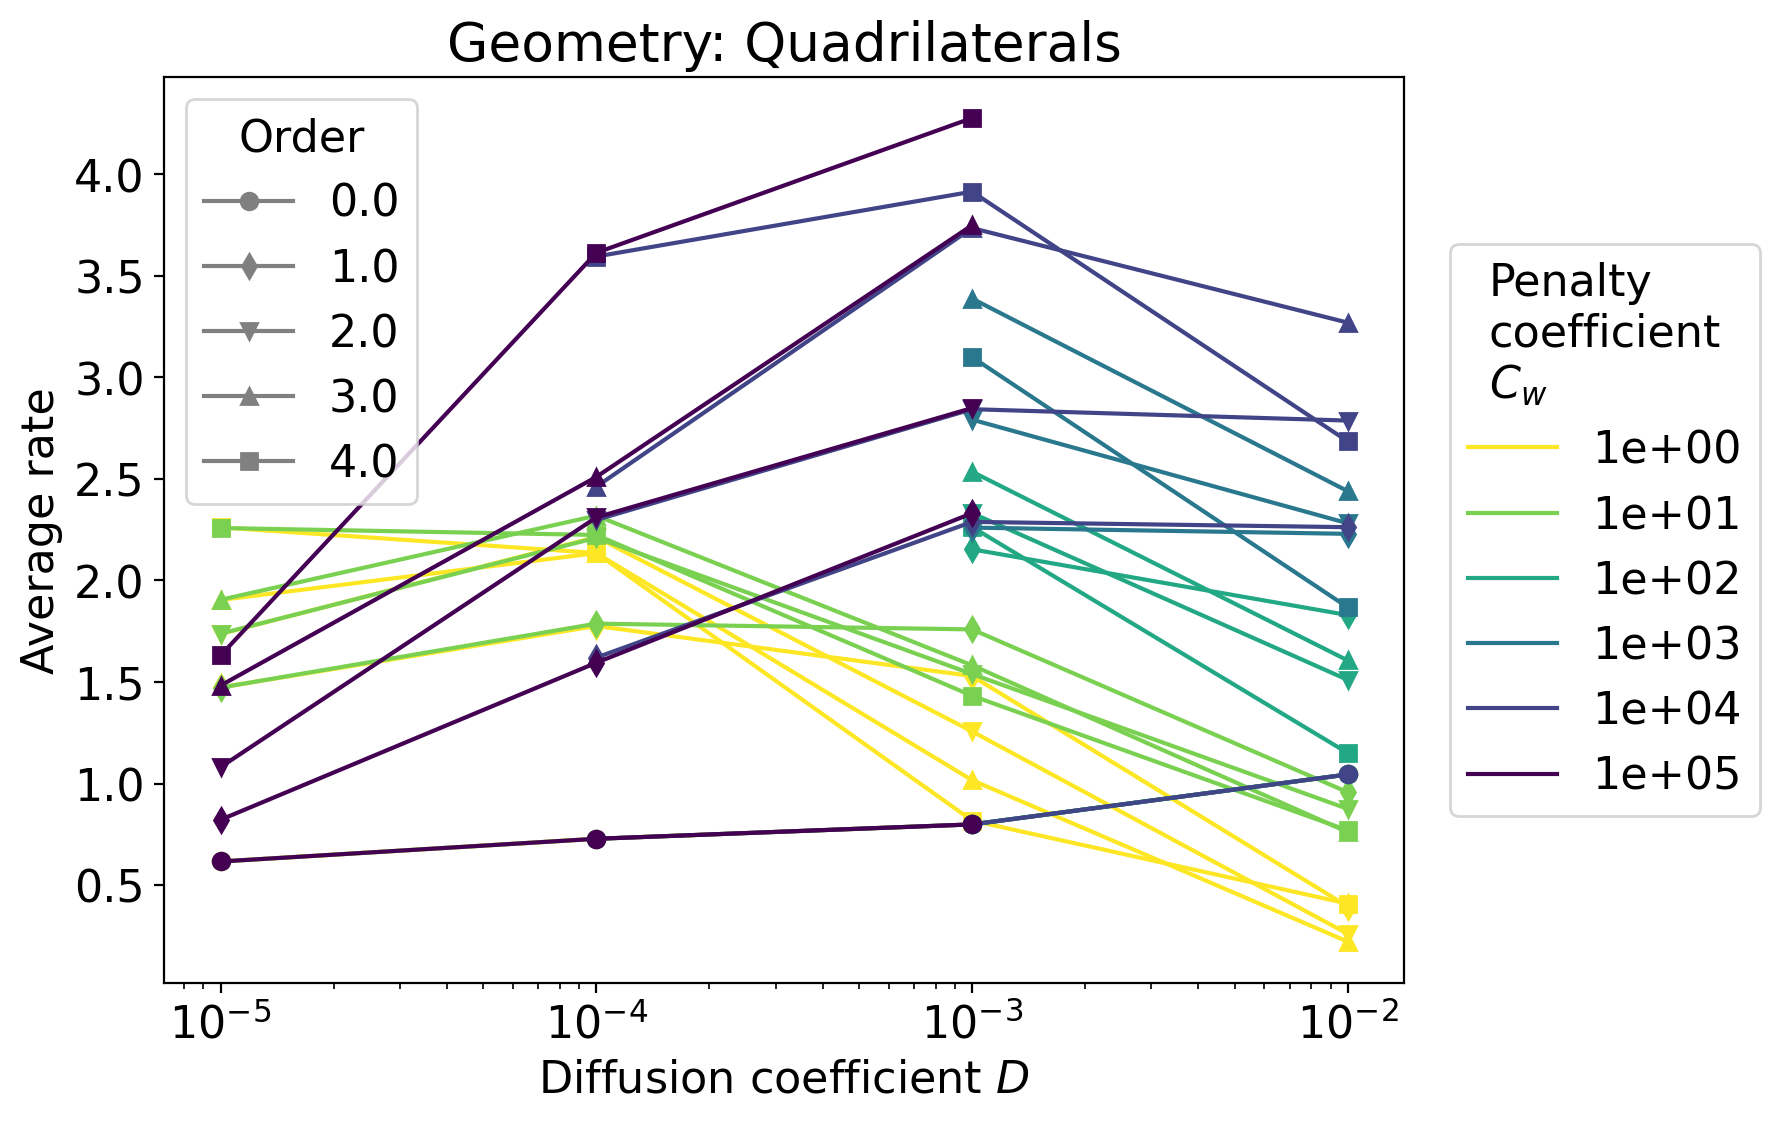
\includegraphics[width=0.49\textwidth]{../figs/parametric/advdiff_2D/ord_quarteroni2_2_4}
	&
	\vspace{0pt} 
	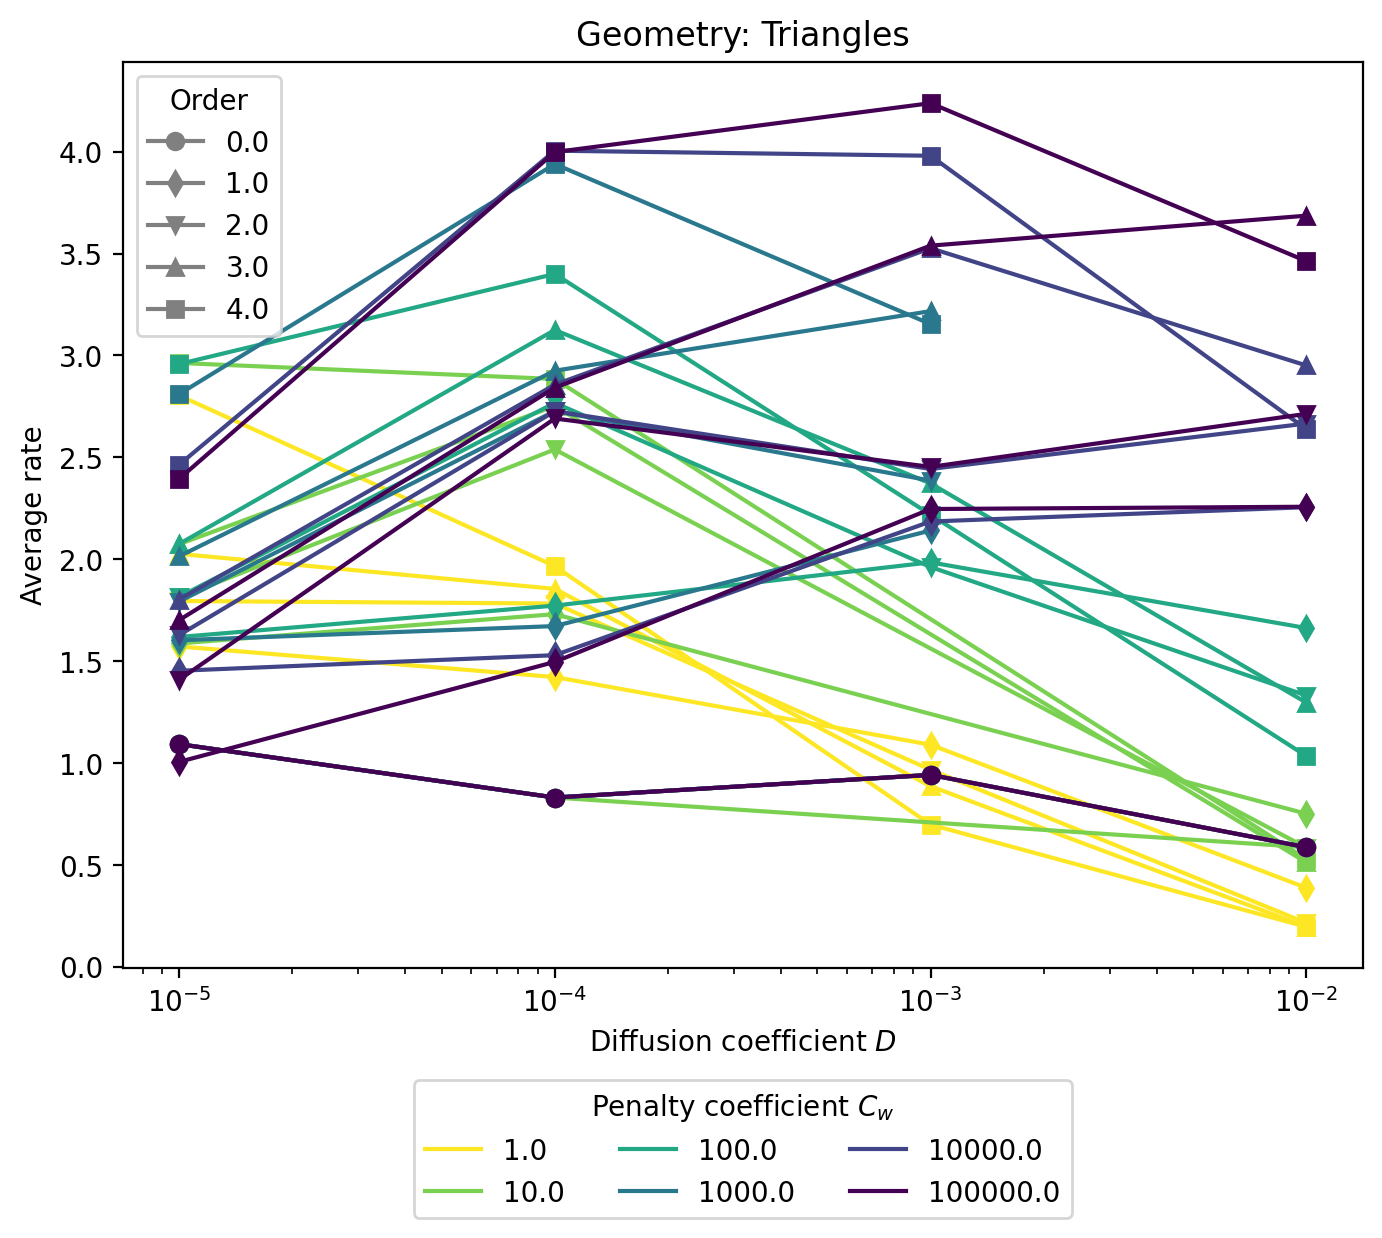
\includegraphics[width=0.49\textwidth]{../figs/parametric/advdiff_2D/ord_quarteroni2_2_3}
	\end{tabular}
	\caption{\Cref{ex:quart3} average order for different choice of $C_w$}
	\label{fig:orders_quarteroni3}
\end{figure}


\begin{figure}[p!]
	\centering
	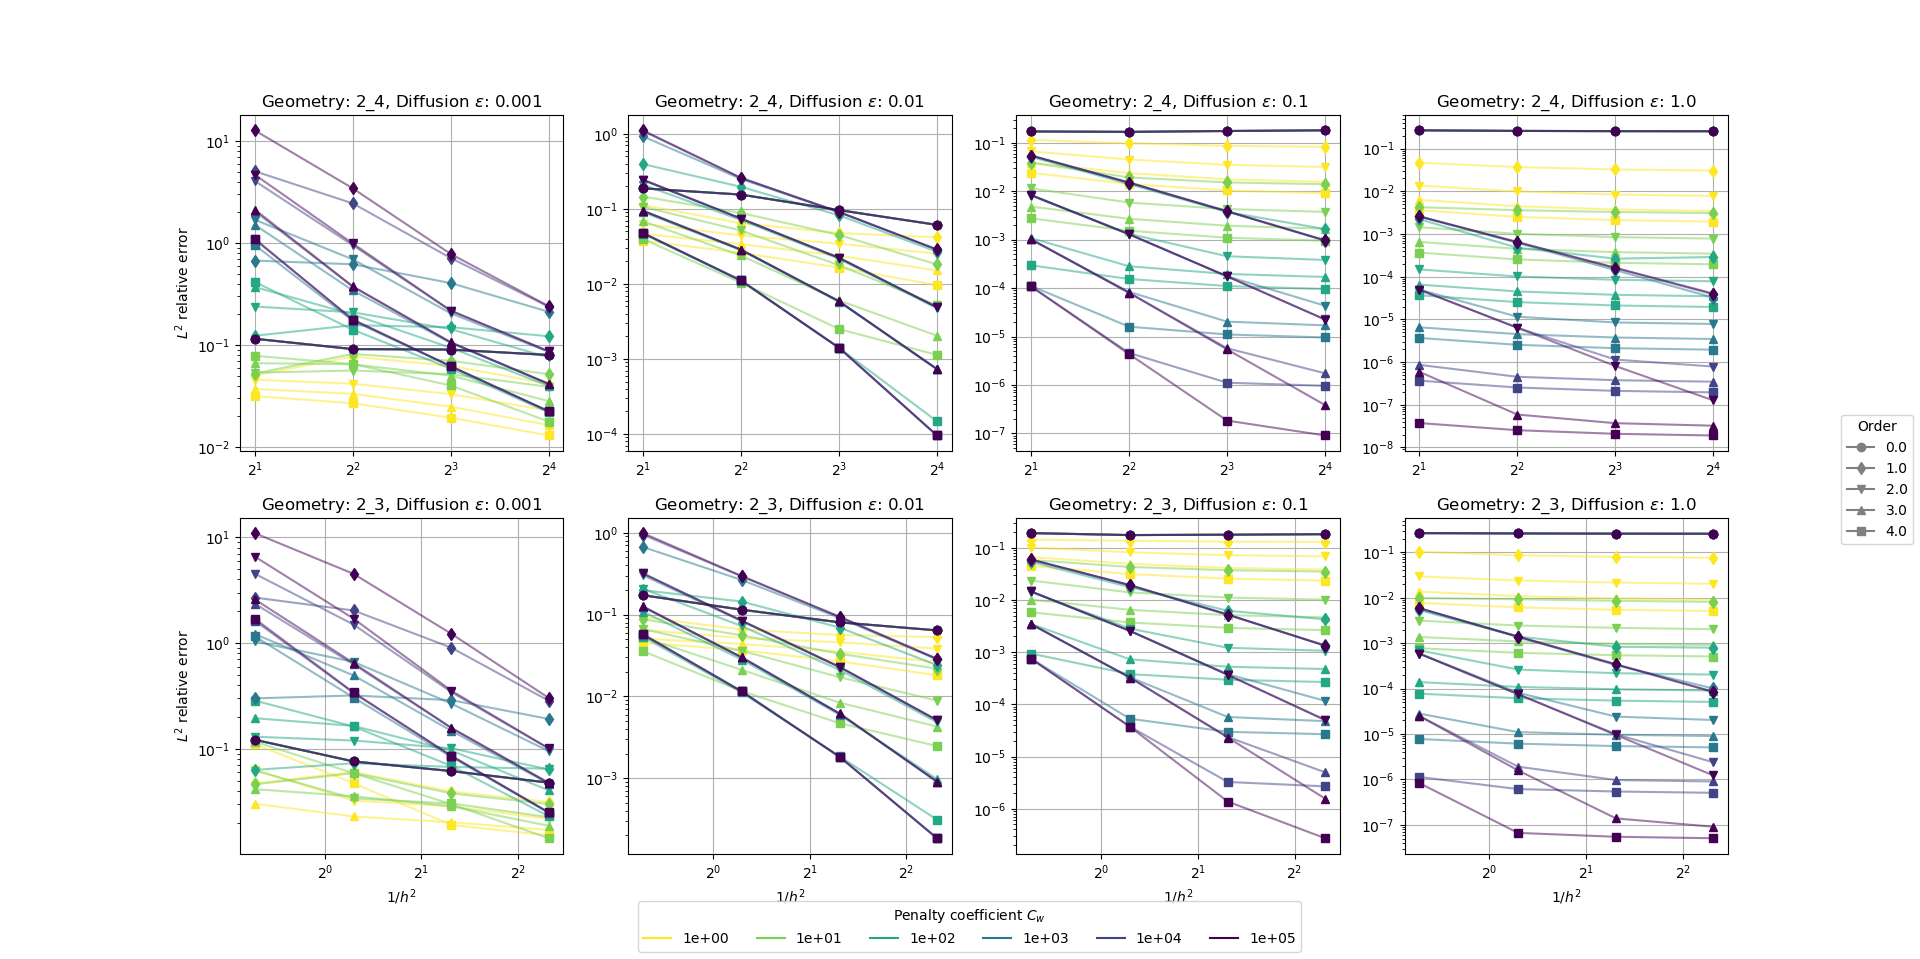
\includegraphics[height=\textheight]{../figs/parametric/advdiff_2D/quarteroni3.png}
	
	\caption{\Cref{ex:quart3} convergence graphs for different choice of $C_w$}
	\label{fig:conv_qart3}
\end{figure}
\newpage
\begin{example}[Advection 1D]
\label{ex:adv1D}
In $\Omega = \langle 0, 1 \rangle$ we will solve equation \eqref{eq:ex_advection}.
%\begin{equation}
%\pdiff{u}{t} + \fdiff{u}{x} = 0.
%\end{equation}
We set two the initial conditions $u(0, x)$ to obtain two different solutions:
\begin{equation}
u_{smooth} = \begin{cases}
g(x),\quad &0.1 < x < .3\\
0, \quad &\text{elsewhere}
\end{cases}
\end{equation}
where
\begin{equation}
g(\xi) = \exp\left(\frac{1}{10(\xi - 0.2)^2 - 1}+ 1\right),
\end{equation}
and
\begin{equation}
u_{step} = \begin{cases}
\dfrac{1}{2},\quad &0.1 < x < .3\\
0, \quad &\text{elsewhere}
\end{cases}.
\end{equation}
And prescribe periodic boundary condition at $x = 0 $ and $x = 1$  this 
results in the solution at time $t = 1$ to be the same as initial condition 
i.e.
\begin{equation}
u(1, x) = u(0, x).
\end{equation} 
%First we evaluate approximation of initial condition. As seen from figure 
%\ref{fig:conv_0adv1D} the approximation corresponds to theoretical orders.
We then compare these to test the convergence, see Figures 
\ref{fig:adv_conv_1D} and \ref{fig:adv_conv_1D_step}. For smooth initial condition 
limiting increases error of the solution due to artificial diffusion, higher order 
methods are capable of counteracting this effect though. For discontinuous initial 
condition limiting significantly improves behavior of the method removing oscillations 
and basically enabling use of high order methods, which suffer from them the most. The 
resulting errors are still significant as limiting introduces prominent 
smoothing. Note that for both $u_{smooth}$ a $u_{step}$ with and without limiting the 
convergence rate of the method is impacted by used 3rd order TVD Runge-Kutta 
time-stepping solver. 
\end{example}

\begin{figure}[h!]
	\centering
	\begin{subfigure}{.5\textwidth}	
		\centering	
		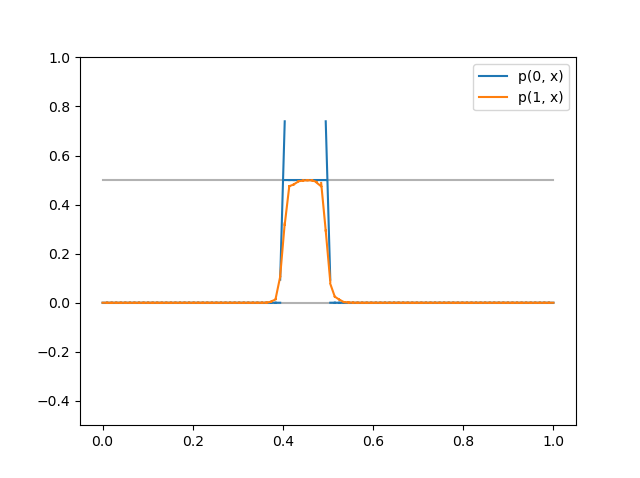
\includegraphics[width=\linewidth]{../figs/sols/adv1d_o2h100_limit}
		\caption{Limit: True}
	\end{subfigure}%
	\begin{subfigure}{.5\textwidth}
		\centering	
		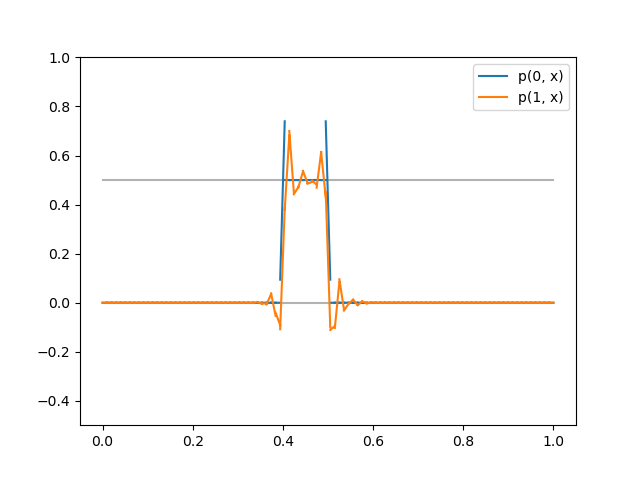
\includegraphics[width=\linewidth]{../figs/sols/adv1d_o2h100_nolimit}
		\caption{Limit: False}
	\end{subfigure}
	\caption{\Cref{ex:adv1D} Solution for $u_{step}$ for CFL coefficient $c=0.1$}
	\label{fig:sol_adv1D} 
\end{figure}

\begin{figure}[p!]
	\centering
	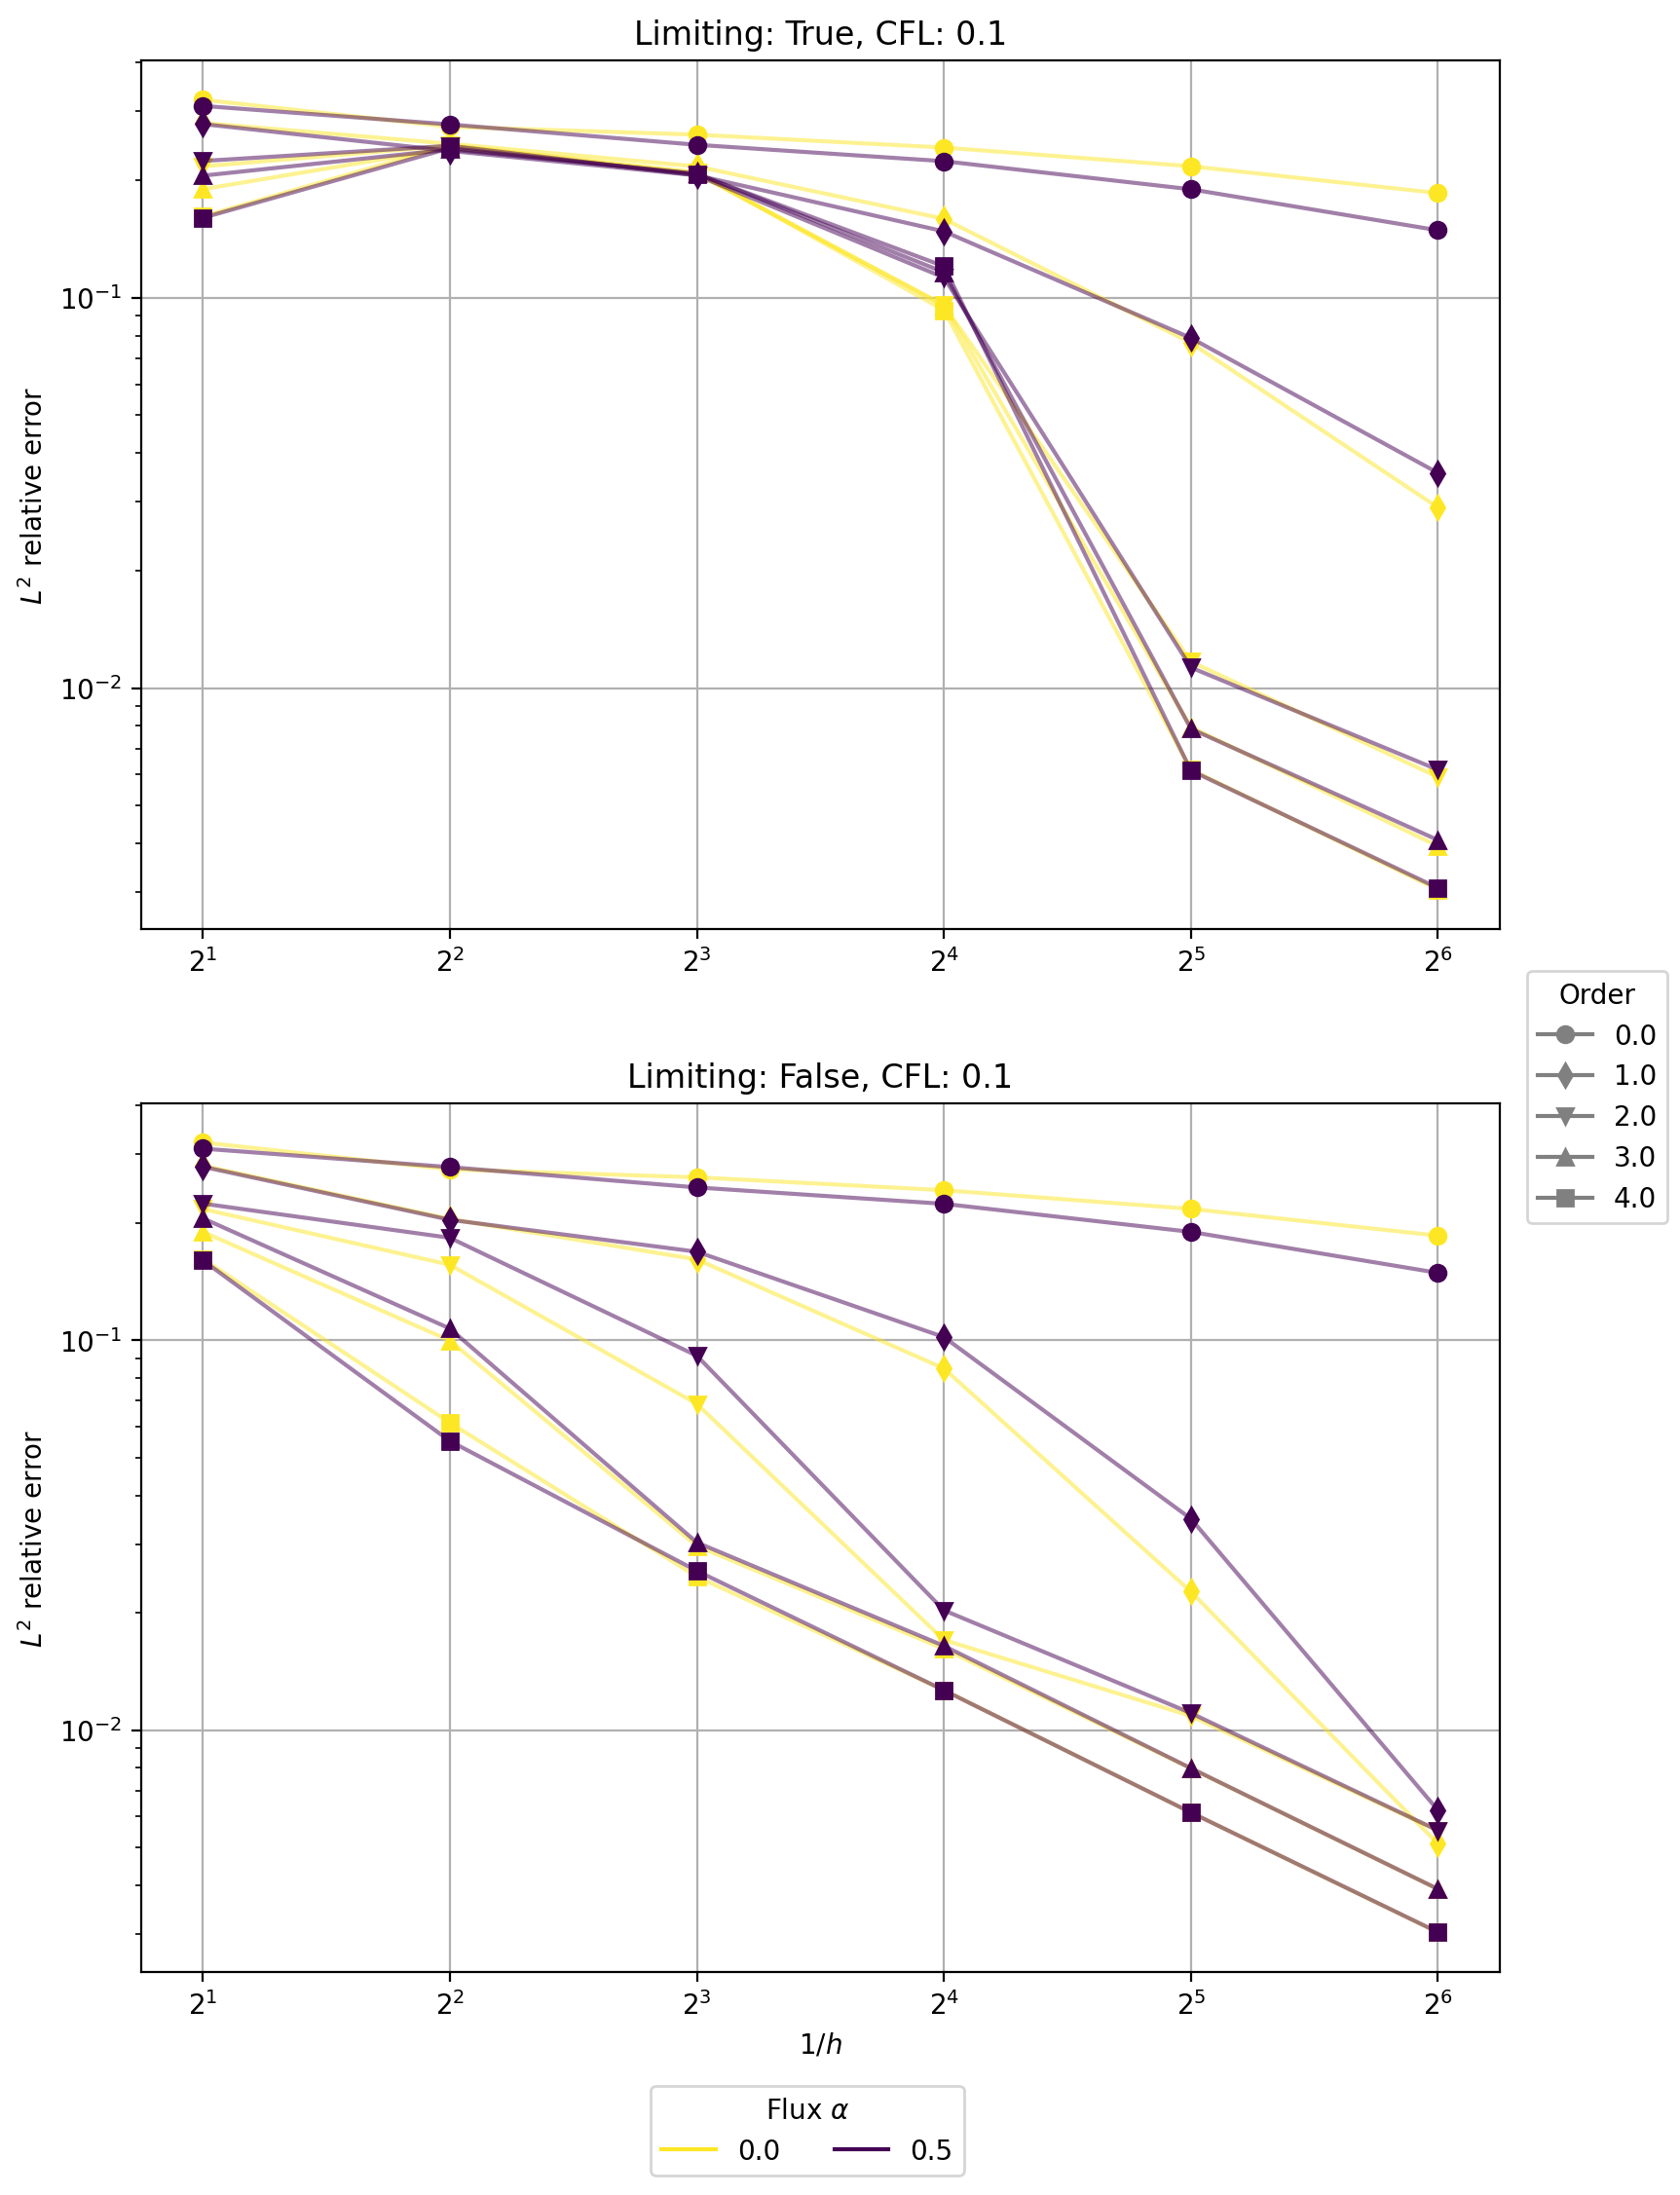
\includegraphics[width=1.1\textwidth]{../figs/parametric/advection_1D/advection_1D_smooth_reduced.png}
	\caption{\Cref{ex:adv1D} convergence plots for smooth initial condition 
		$u_{smooth}$}
	\label{fig:adv_conv_1D}
\end{figure}


\begin{figure}[p!]
	\centering
	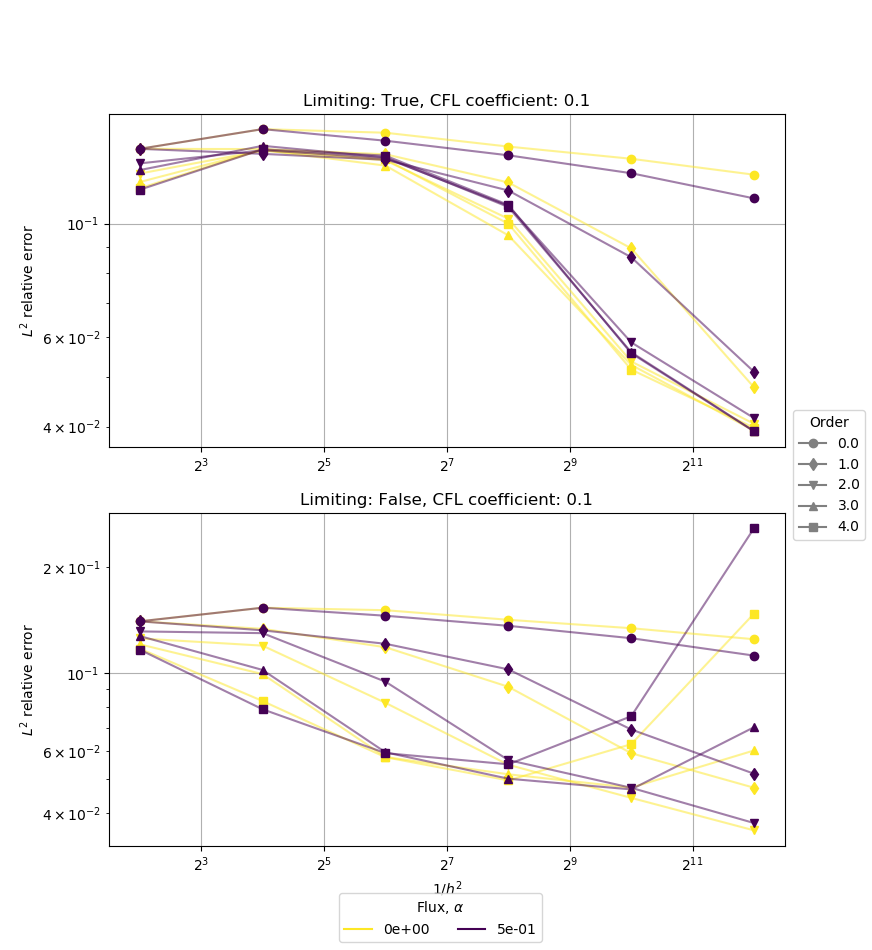
\includegraphics[width=1.1\textwidth]{../figs/parametric/advection_1D/advection_1D_step_reduced.png}
	\caption{\Cref{ex:adv1D} convergence plots for discontinuous initial 
	condition $u_{step}$}
	\label{fig:adv_conv_1D_step}
\end{figure}


\newpage
\section{Diffusion}
%\newpage
\paragraph{Example 10}
In $\Omega = \langle 0, 1 \rangle$ we will solve Poisson equation
\begin{equation}
\varepsilon \cdot \pdiff{^2 u}{x^2} = g
\end{equation}
where  $\varepsilon$ is diffusion coefficient and $g$ a source function. We setup boundary conditions and source 
function in such way that the exact solution $u_{exact}$ is
\begin{equation}
u_{exact} = \sin(2\pi x)
\end{equation}
Solving for $g$ yields
\begin{equation}
	g = 4\pi^2\varepsilon\sin(2\pi x)
\end{equation}
We set boundary conditions to match analytical solution as follows
\begin{equation}
	\begin{aligned}
		&u(0) = 0,      &u(1) = 0\\
		&u_x(0) = 2\pi, &u_x(1) = 2\pi.
	\end{aligned}
\end{equation}

Again different values of coefficient $Cw$ in penalty term then yield different convergence behavior as demonstrated in 
Figure \ref{fig:conv_diff1D}

\begin{figure}[h]
	\begin{minipage}[b]{0.5\linewidth}
		\includegraphics[width=\textwidth]{../figs/convs/diff1D-cells-cw10_d1_t2}
	\end{minipage}
	\begin{minipage}[b]{0.5\linewidth}
		\includegraphics[width=\textwidth]{../figs/convs/diff1D-cells-cw100_d1_t2}
	\end{minipage}

	\begin{minipage}[b]{0.5\linewidth}
		\includegraphics[width=\textwidth]{../figs/convs/diff1D-cells-cw1000_d1_t2}
	\end{minipage}
	\begin{minipage}[b]{0.5\linewidth}
		\includegraphics[width=\textwidth]{../figs/convs/diff1D-cells-cw10000_d1_t2}
	\end{minipage}
	
	\caption{Example 10 Convergence graph for different choice of $C_w$}
	\label{fig:conv_diff1D}
\end{figure}

To demonstrate what is going on with the error we include plots of numerical solution, exact solution and their 
absolute difference, see Figure \ref{fig:diff1D_sol-err}. For higher orders the solution remains relatively smooth, 
without any oscillations or irregularities, however it gets "overblown".
%\begin{figure}[h]
%	\centering
%	\includegraphics[scale=.25]{../figs/err-sols/diff1D-err-sol-i20cw1_d1_t2}
%	\includegraphics[scale=.25]{../figs/err-sols/diff1D-err-sol-i20cw100_d1_t2}
%	\includegraphics[scale=.25]{../figs/err-sols/diff1D-err-sol-i20cw10000_d1_t2}
%	\caption{Example 10 Exact solution (gray), numerical solution (orange) and their absolute difference (red) for 
%		different orders and $h$. The left $y$ axes correspond to the solutions, the right ones to their difference.}
%	\label{fig:diff1D_sol-err}
%\end{figure}
%\newpage
\paragraph{Example 2} Based on [Hartmann]
On $\Omega = \langle 0, 1 \rangle^2$ we will poisson equation
\begin{equation}
\varepsilon \cdot \left( \pdiff{^2 u}{x^2} + \pdiff{^2 u}{y^2} \right) = g
\end{equation}
i.e
\begin{equation}
- \varepsilon \Delta u = g
\end{equation}
where  $\varepsilon$ is diffusion coefficient and $g$ is a source 
function. We setup boundary condition and source function in such way that the exact solution $u_{exact}$ is
\begin{equation}
u_{exact} =  \sin\left(\frac{1}{2} \, \pi x_{1}\right) \sin\left(\frac{1}{2} \, \pi x_{2}\right)
\end{equation}
Solving for $g$ yields
\begin{equation}
\begin{aligned}
	g = \frac{1}{2} \, \pi^{2} \varepsilon \sin\left(\frac{1}{2} \, \pi x_{1}\right) \sin\left(\frac{1}{2} \, \pi 
		x_{2}\right) +\\ \frac{1}{2} \, \pi \cos\left(\frac{1}{2} \, \pi x_{2}\right) \sin\left(\frac{1}{2} \, \pi 
		x_{1}\right) + \\\frac{1}{2} \, \pi \cos\left(\frac{1}{2} \, \pi x_{1}\right) \sin\left(\frac{1}{2} \, \pi 
		x_{2}\right)
\end{aligned}
\end{equation}
We set boundary conditions to match analytical solution.
Again different values of coefficient $Cw$ in penalty term then yield different convergence behavior as demonstrated in 
Figure \ref{fig:conv2}

\begin{figure}[ht]
	\begin{minipage}[b]{0.5\linewidth}
		\includegraphics[width=\textwidth]{../figs/diffusion_only_hartmann-cells-cw10_d1}
	\end{minipage}
	\begin{minipage}[b]{0.5\linewidth}
		\includegraphics[width=\textwidth]{../figs/diffusion_only_hartmann-cells-cw100_d1}
	\end{minipage}

	\begin{minipage}[b]{0.5\linewidth}
		\includegraphics[width=\textwidth]{../figs/diffusion_only_hartmann-cells-cw1000_d1}
	\end{minipage}
	\begin{minipage}[b]{0.5\linewidth}
		\includegraphics[width=\textwidth]{../figs/diffusion_only_hartmann-cells-cw10000_d1}
	\end{minipage}
	
	\caption{Example 2 Convergence graph for different choice of $C_w$}
	\label{fig:conv2}
\end{figure}
\begin{example}[Diffusion 2D]
\label{ex:laplace}
Inspired by \cite[cv. 8.4 (3), p. 150]{Holubova2011}, in $\Omega = \langle 0, 1 
\rangle^2$ 
we will solve Laplace equation \eqref{eq:ex_laplace}.
%\begin{equation}
%\pdiff{^2 u}{x^2} + \pdiff{^2 u}{y^2} = 0
%\end{equation}
%i.e
%\begin{equation}
%\Delta u = 0.
%\end{equation}
We setup boundary condition in such way that the exact solution 
$u_{exact}$ is polynomial
\begin{equation}
u_{exact} = \frac{1}{2}x^2 - \frac{1}{2}y^2 - ax + by + c.
\end{equation}
We set boundary conditions to match analytical solution as follows
\begin{equation}
	\begin{aligned}
		&u_x(0, y) = -a, & u_x(a, y) = 0\\
		&u_y(x, 0) = b, & u_y(x, b) = 0.
	\end{aligned}
\end{equation}
In our setting we chose $a=1$, $b=1$, $c=0$. Different values of 
coefficient $C_w$ in penalty term yield different convergence behavior as demonstrated in 
Figures \ref{fig:conv_laplace} and \ref{fig:orders_lapalce}.  \Cref{fig:orders_lapalce} 
may suggest that high order method do not meet expected convergence rate, they however 
still attain lowest error as illustrated in \Cref{fig:conv_laplace}. This is due to 
the polynomial solution which can be approximated very accurately even on coarse mesh and 
refining does not provide much benefit especially for high order approximations.
\end{example}

\begin{figure}[h!]
	\centering
	\begin{tabular}{p{0.5\textwidth} p{0.5\textwidth}}
		\vspace{0pt} 
        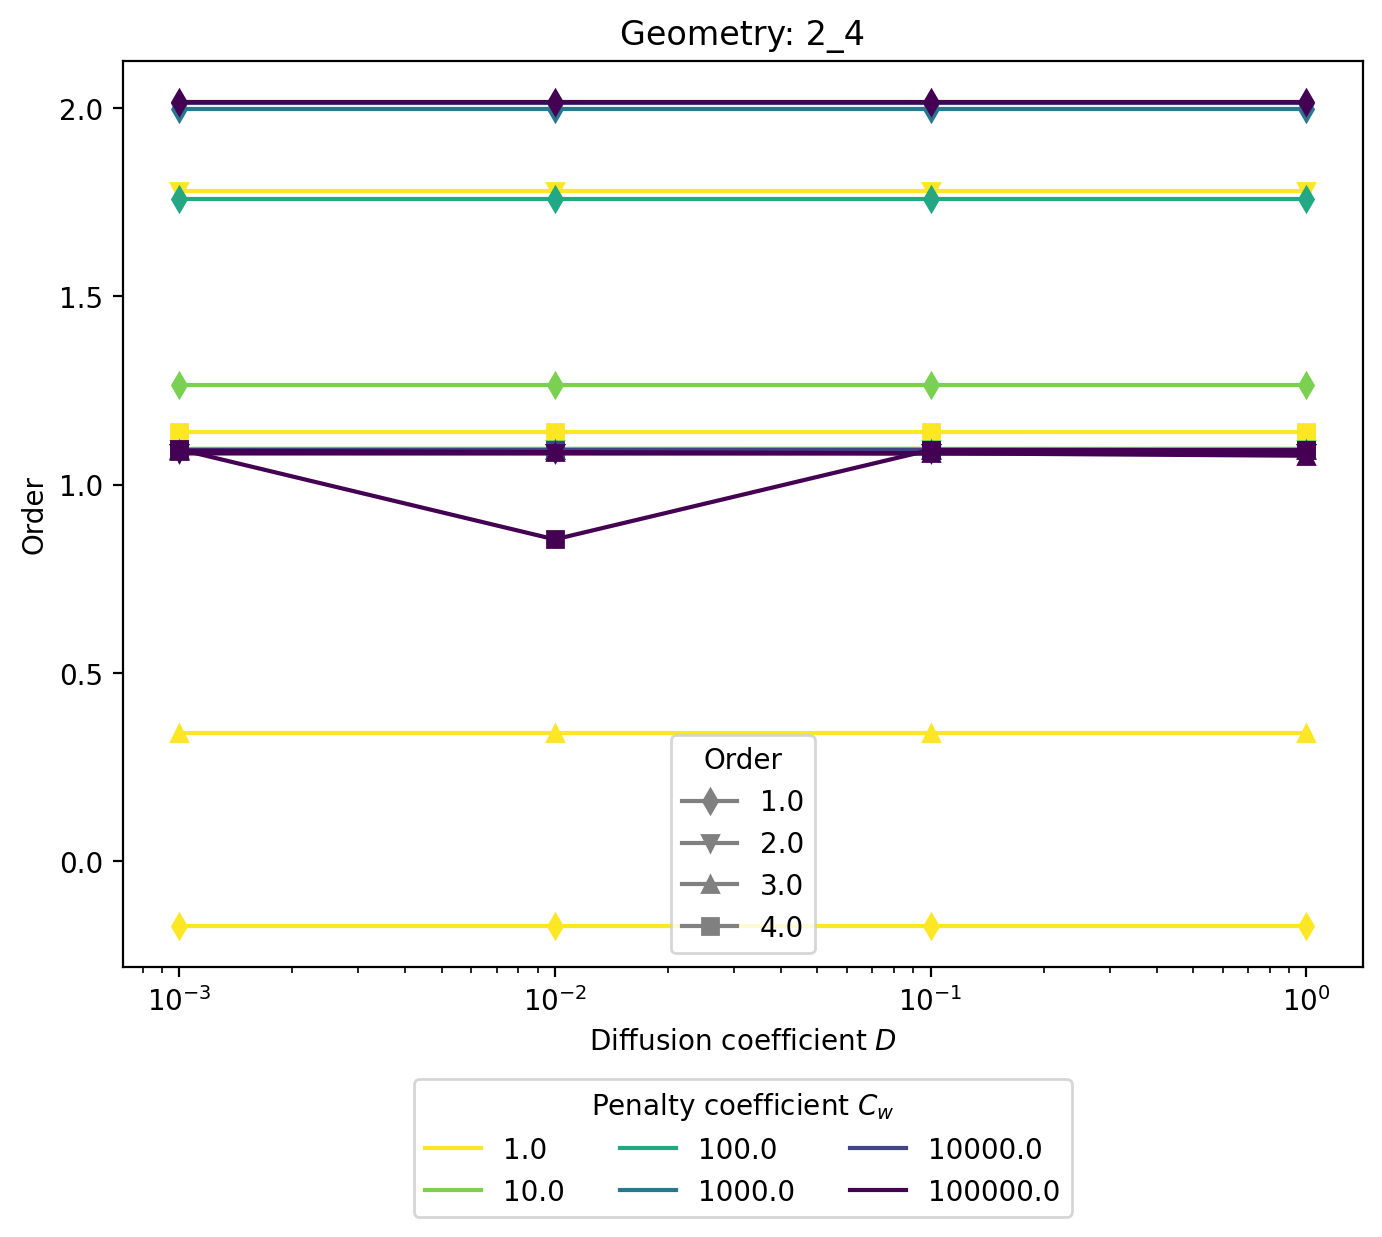
\includegraphics[width=0.49\textwidth]{../figs/parametric/diffusion_2D/ord_laplace_2_4}
		&
		\vspace{0pt} 
        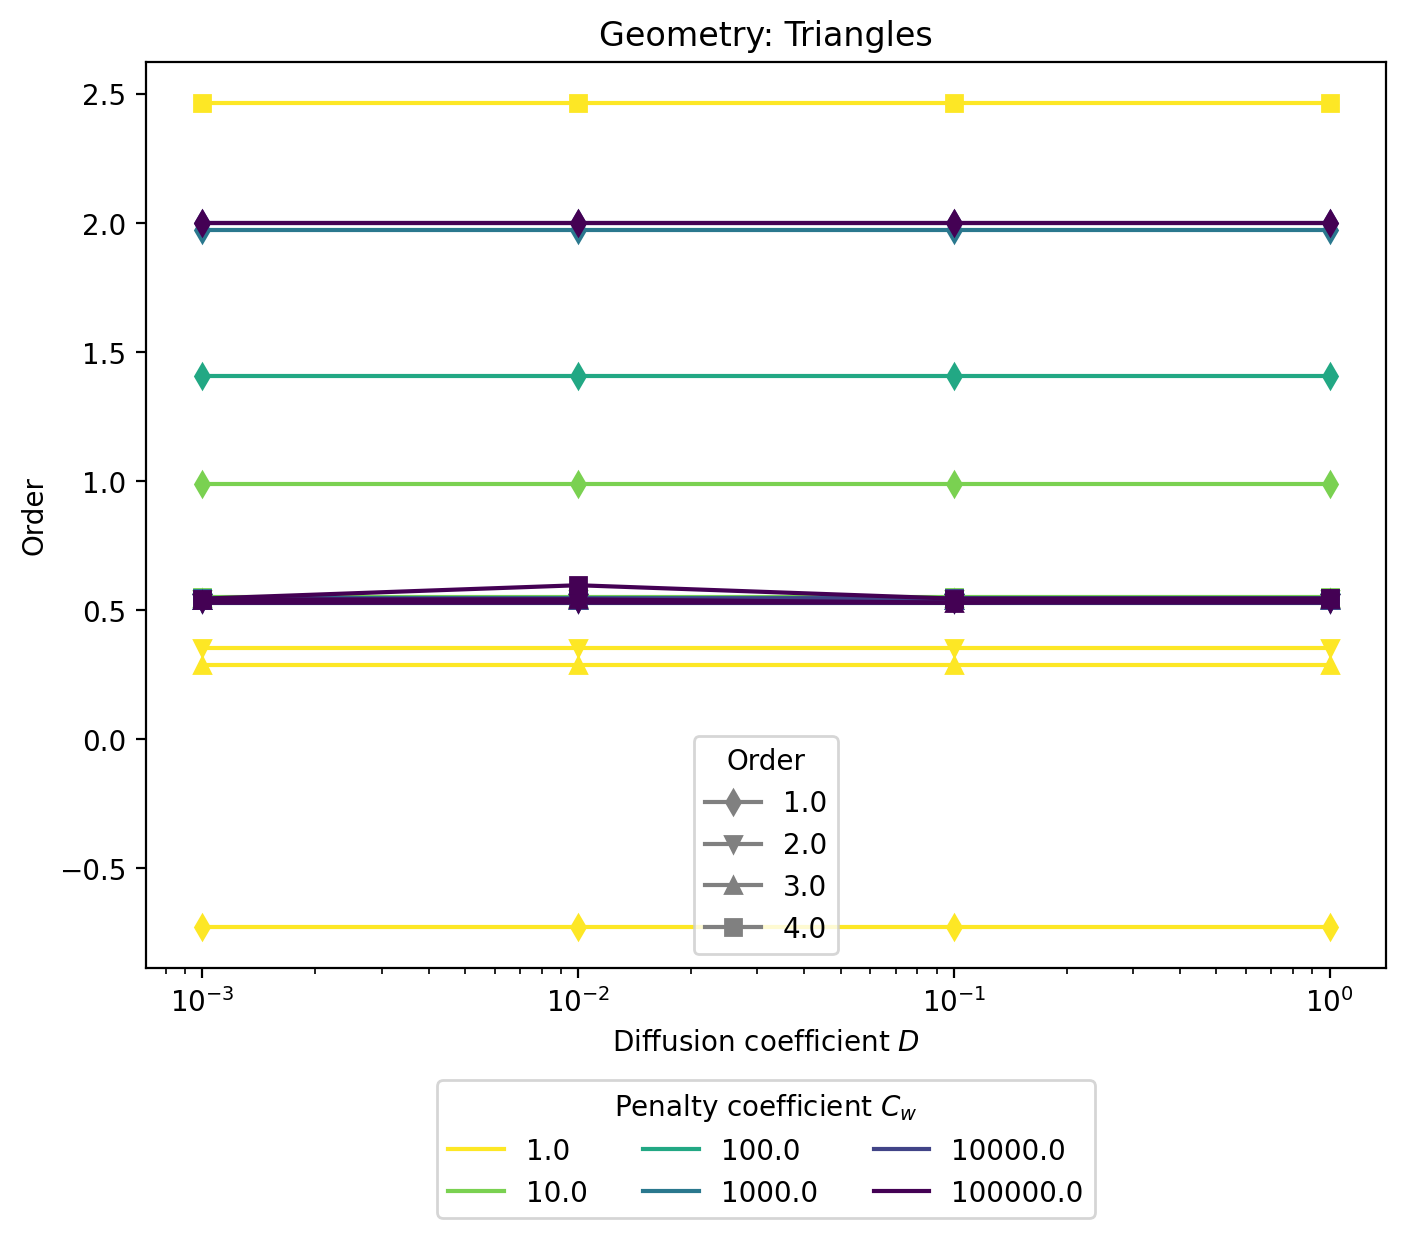
\includegraphics[width=0.49\textwidth]{../figs/parametric/diffusion_2D/ord_laplace_2_3}
	\end{tabular}
	\caption{\Cref{ex:laplace}. Average convergence rates for different choices of $C_w$ 
	for quadrilaterals (left) and triangles (right).}
	\label{fig:orders_lapalce}
\end{figure}

%\begin{figure}[h!]
%	\centering
%	\begin{subfigure}{.5\textwidth}	
%		\centering		
%        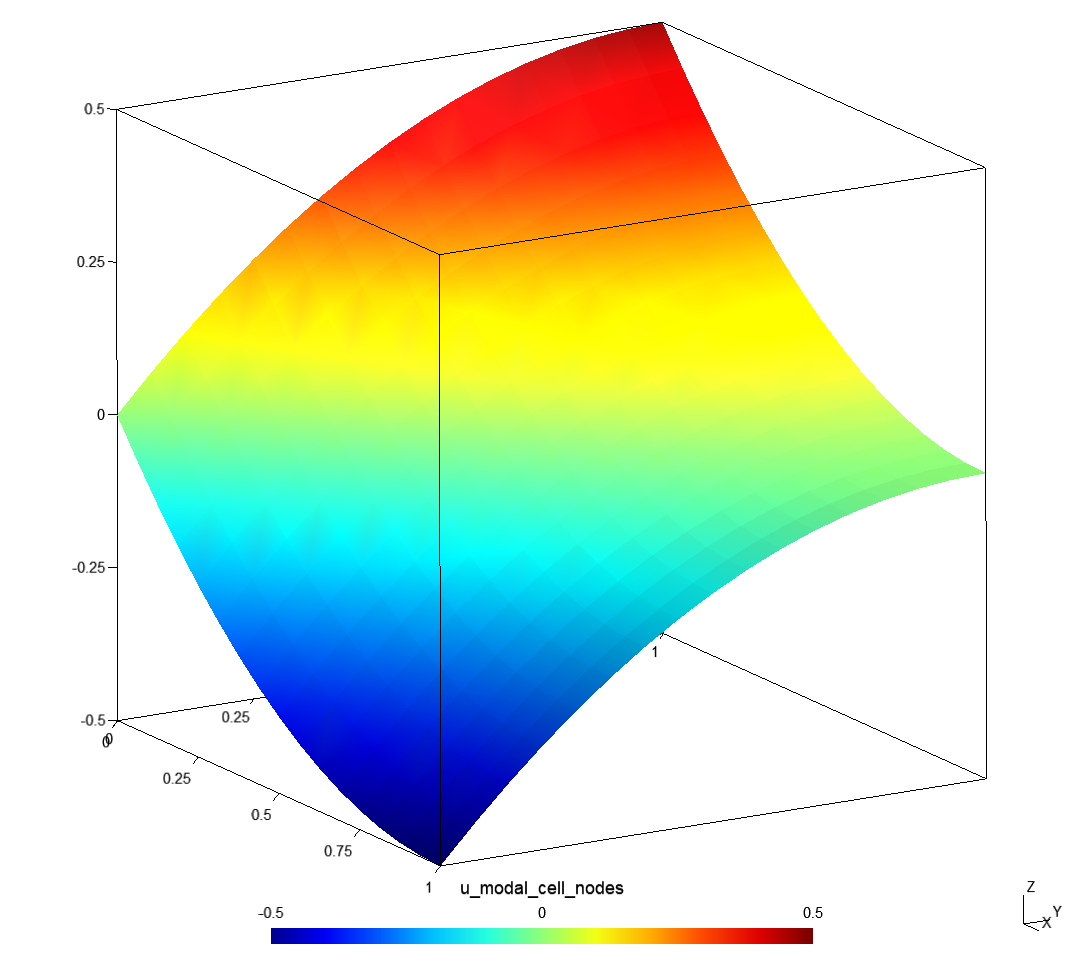
\includegraphics[width=\linewidth]{../figs/sols/laplace-52000-sol-h256o03.png}
%		\caption{??}
%	\end{subfigure}%
%%	\begin{subfigure}{.5\textwidth}
%%		\centering	
%%\includegraphics[width=\linewidth]{../figs/sols/}
%%		\caption{$C_w = 15$}
%%	\end{subfigure}
%	\caption{Solutions of \Cref{ex:laplace}  }
%\end{figure}

\begin{figure}[p!]
	\centering
	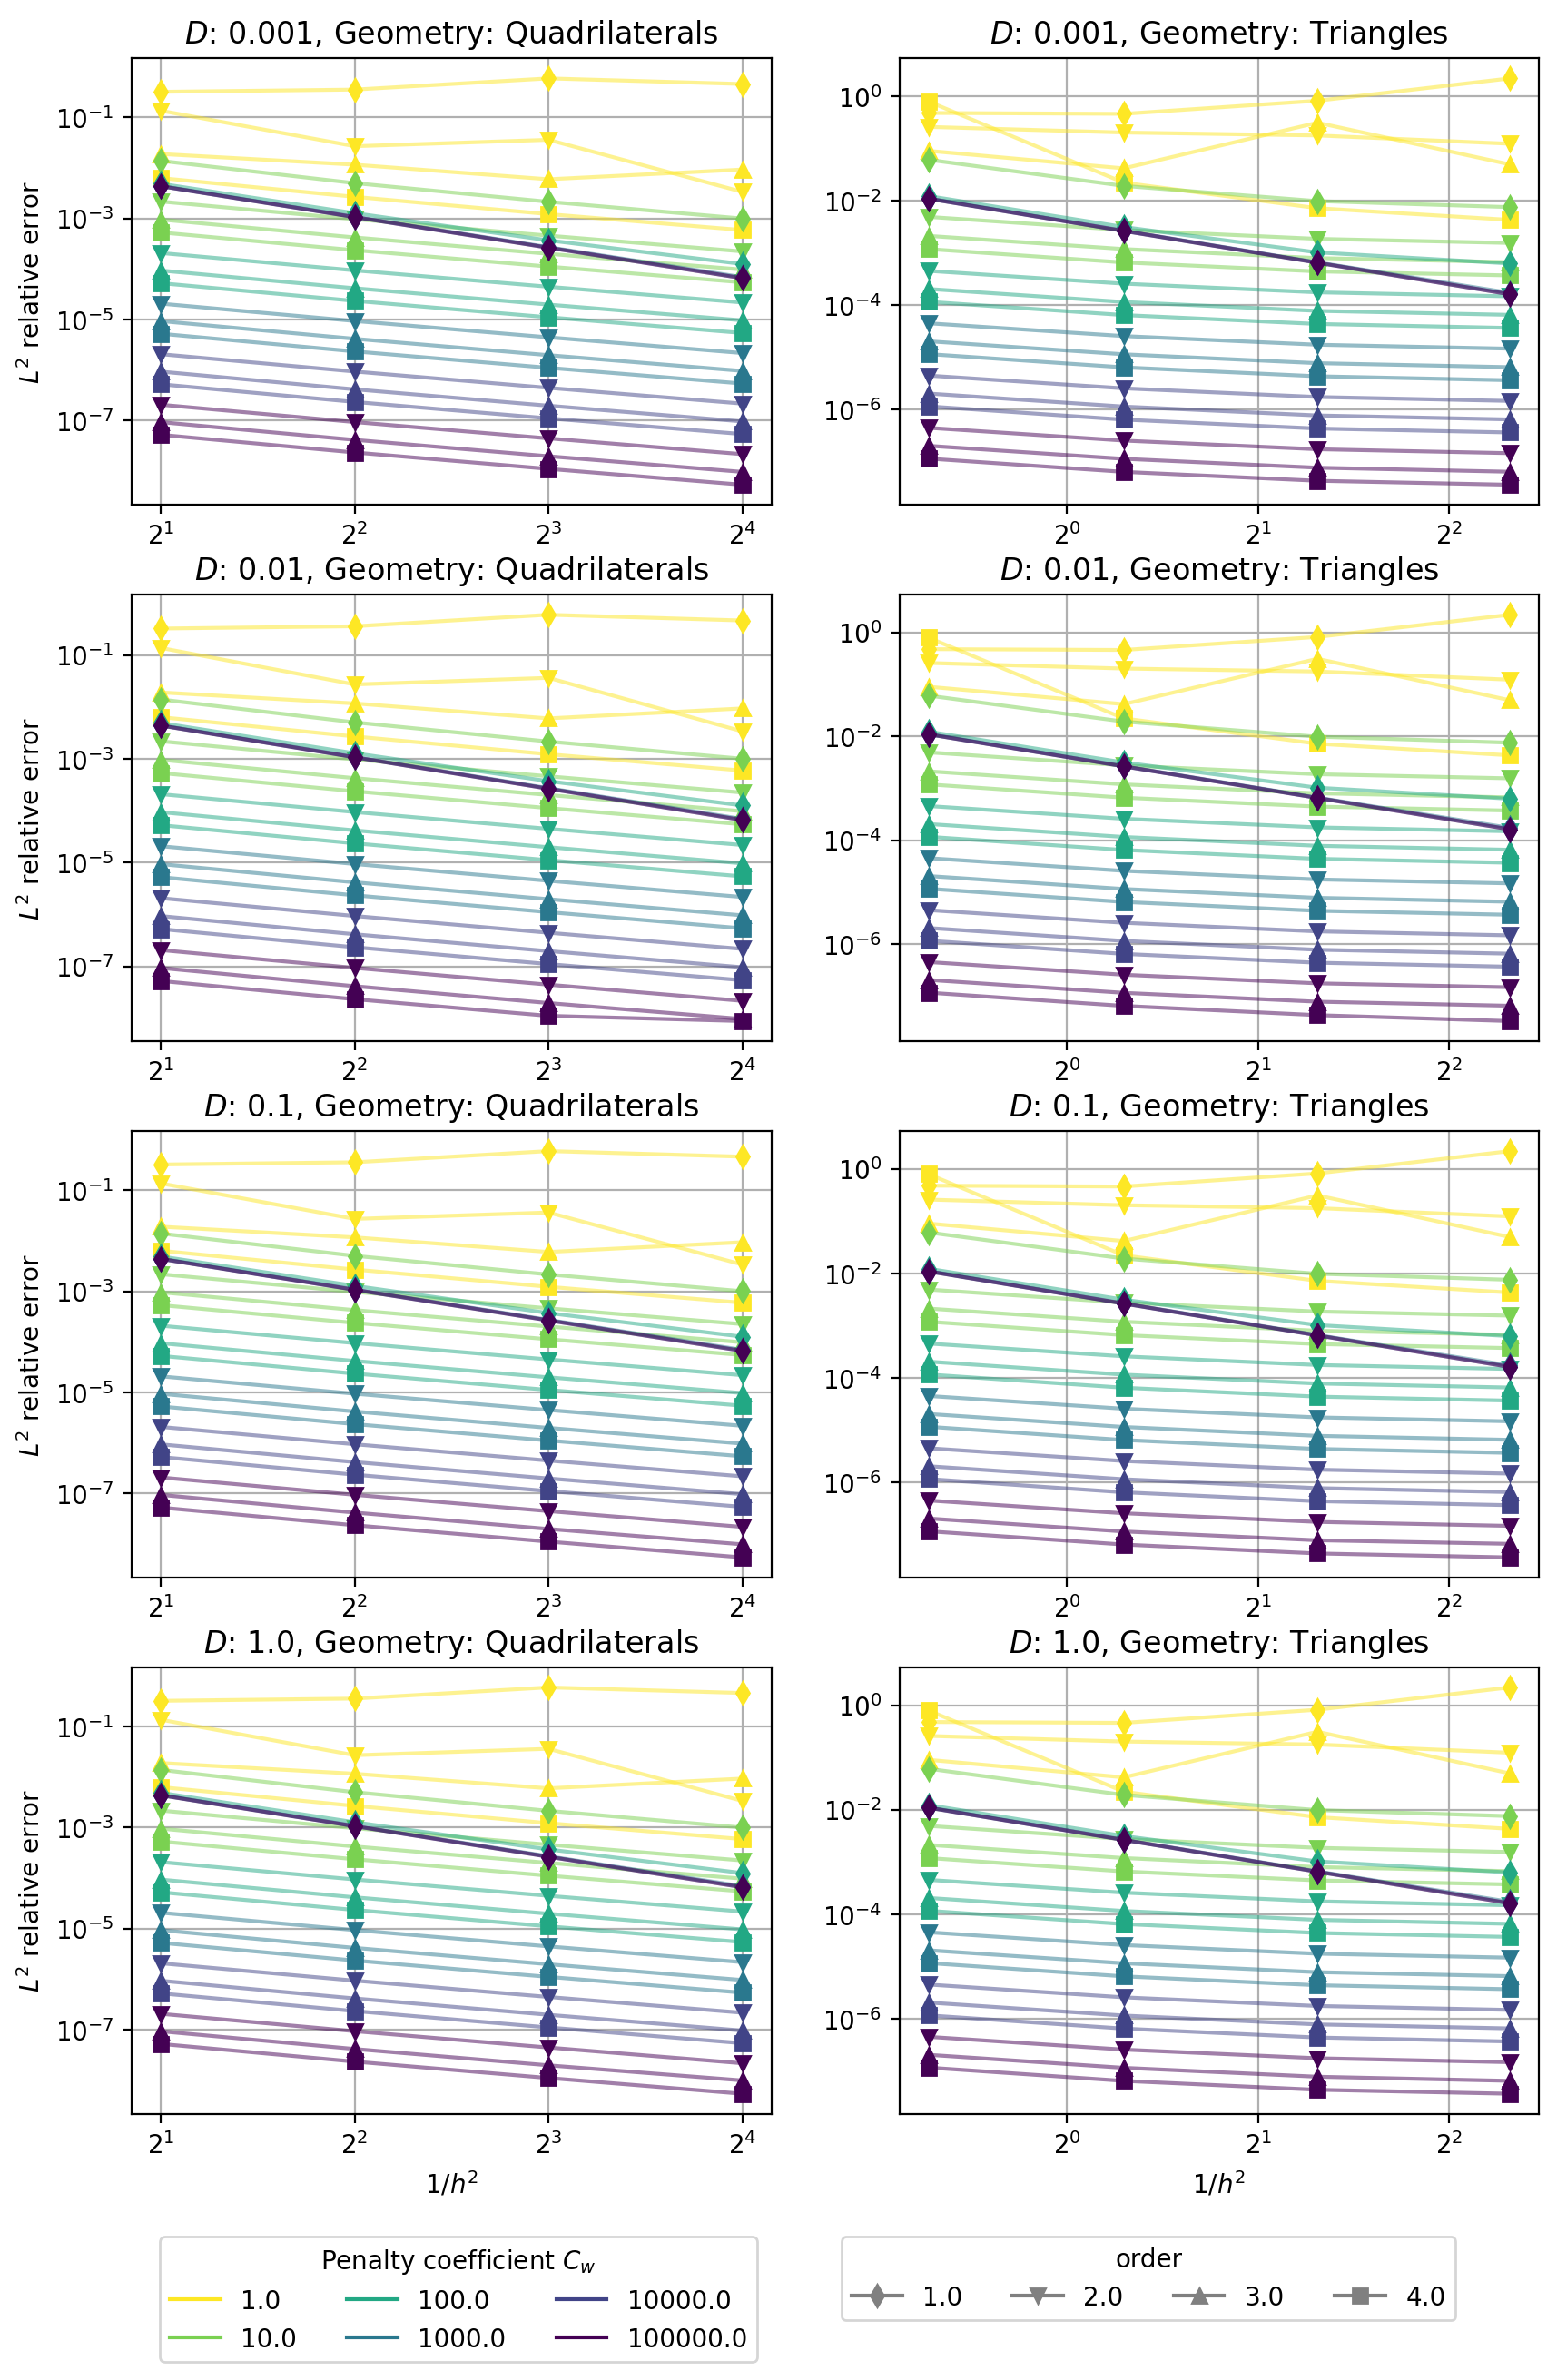
\includegraphics[height=\textheight]{../figs/parametric/diffusion_2D/laplace.png}
	\caption{\Cref{ex:laplace}. Relative errors for different choice of $C_w$  for 
		quadrilaterals (left) and triangles (right).}
	\label{fig:conv_laplace}
\end{figure}

\newpage
\section{Burgess with diffusion}
%\begin{example}[Viscous Burgers 2D]
\label{ex:kucera}
Based on example in \cite[Section 1.6]{Kucera},
we will solve equation \eqref{eq:ex_burgers} in $\Omega = \langle 0, 1 \rangle^2$.
%\begin{equation}
%		\pdiff{u}{t} + \frac{1}{2}\left(\pdiff{u^2}{x} + \pdiff{u^2}{y}\right)  - 
%		D \cdot \left( \pdiff{^2 u}{x^2} + \pdiff{^2 u}{y^2} \right) 
%		= g
%\end{equation}
%where $D$ is diffusion coefficient and $g$ is a source function. 
We setup boundary condition and source function in such way that the exact 
solution $u_{exact}$ is
\begin{equation}
	u_{exact} =  \ -{\left(e^{\left(-t\right)} - 1\right)} {\left(\sin\left(5 \,x 
	y\right) + \sin\left(-4 \, 
	x y + 4 \,x + 4 \, y\right)\right)}.
\end{equation}
We omit analytical forms of $g$ and boundary conditions for brevity.
Different values of coefficient $C_w$ in penalty term then yield only slightly different 
convergence behavior as demonstrated in Figure \ref{fig:kucera_conv} and 
\Cref{fig:kucera_orders}. In this case the solution does not feature any sharp steps and 
increase in penalty coefficient leads to increase in accuracy. In \Cref{fig:sol_kucera} 
this effect is clearly visible in sample solution, similarly to \Cref{ex:quart1}. Kučera 
in \cite{Kucera} reports average convergence rates for irregular triangular mesh 
slightly higher then ours.

\end{example}
\begin{figure}[h!]
	\centering
	\begin{tabular}{p{0.5\textwidth} p{0.5\textwidth}}
		\vspace{0pt} 
		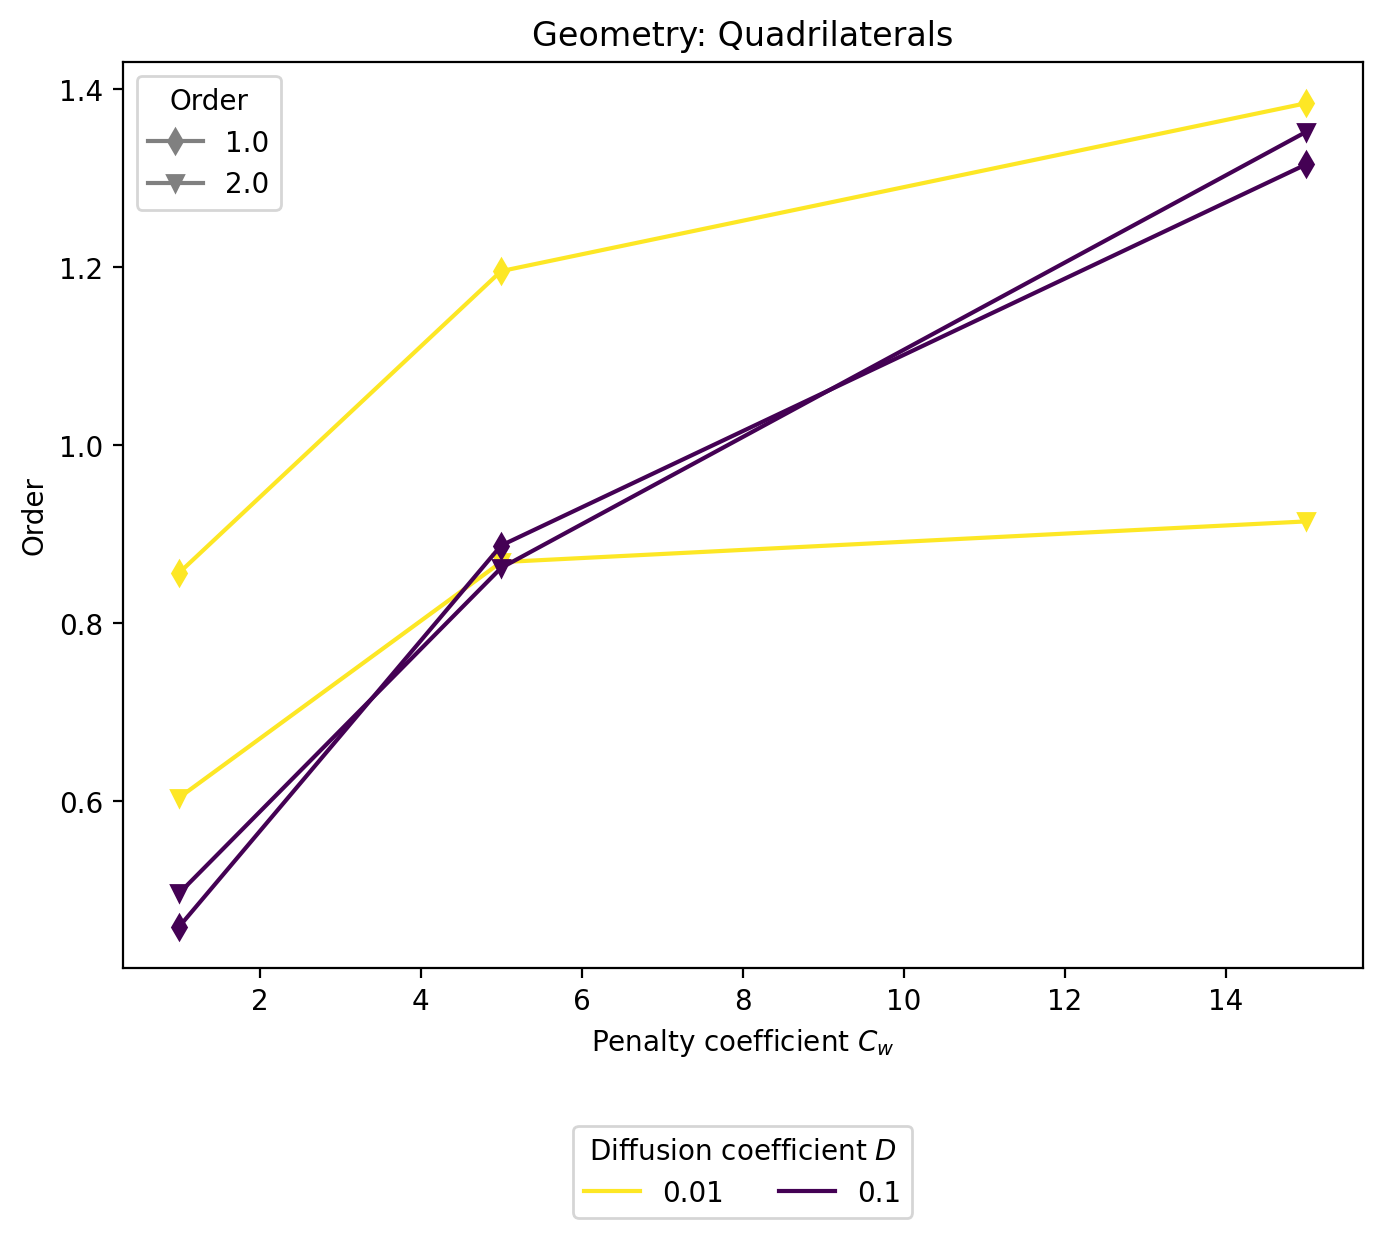
\includegraphics[width=0.49\textwidth]{../figs/parametric/burgers_2D/orders_2_4}
		&
		\vspace{0pt} 
		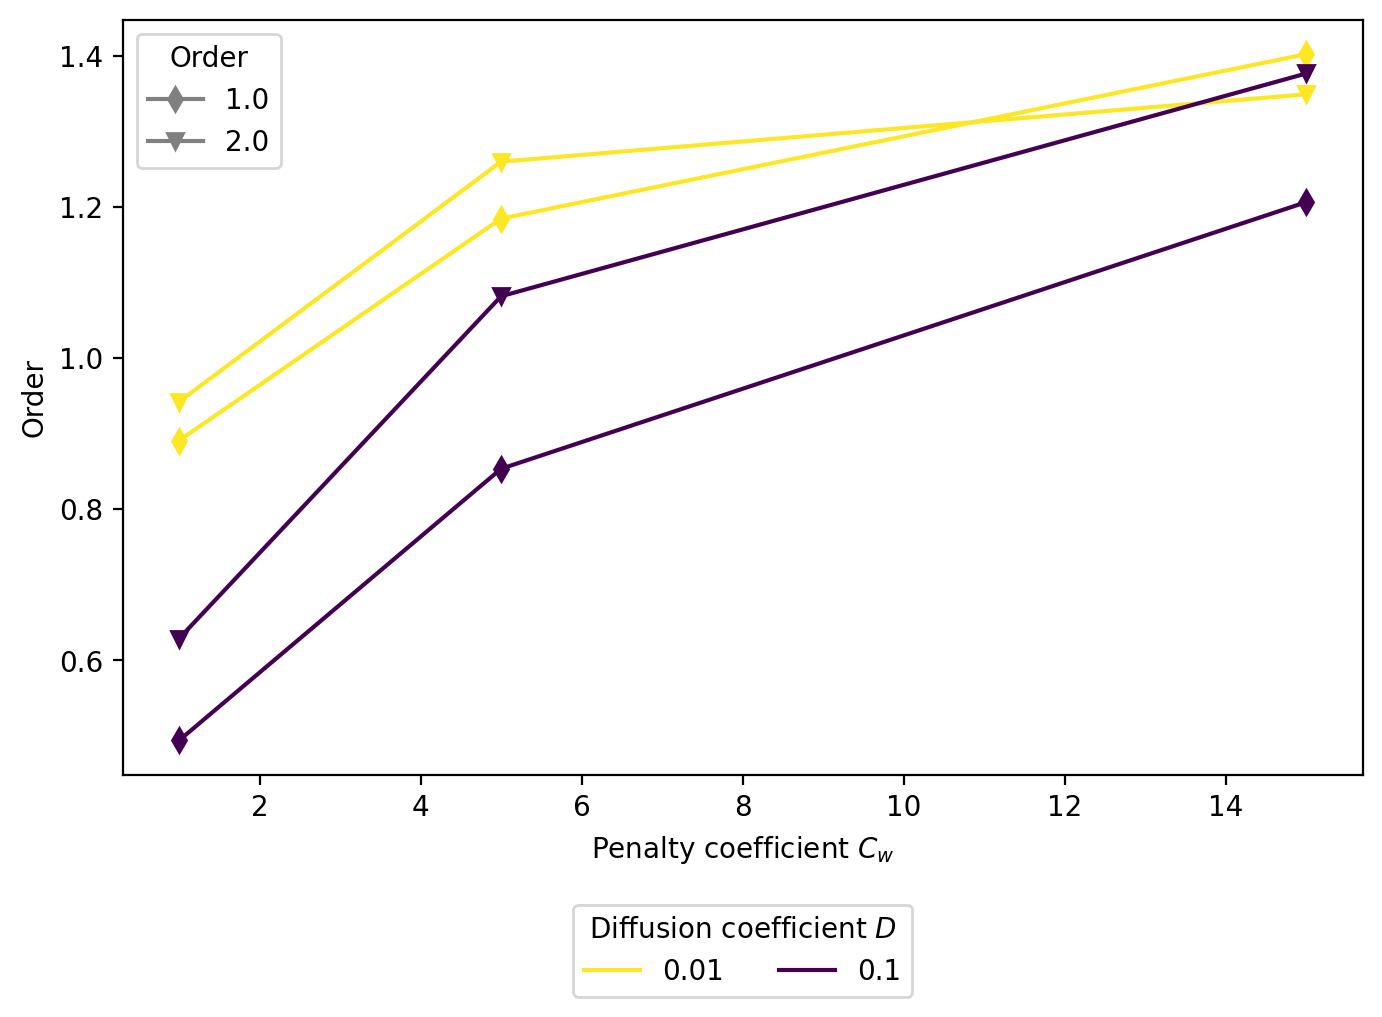
\includegraphics[width=0.49\textwidth]{../figs/parametric/burgers_2D/orders_2_3}
	\end{tabular}
	\caption{\Cref{ex:kucera}. Average orders for different values of $C_w$ for 
	quadrilaterals (left) and triangles (right).}
	\label{fig:kucera_orders}
\end{figure}


\begin{figure}[h!]
	\centering
	\begin{subfigure}{.5\textwidth}	
		\centering	
		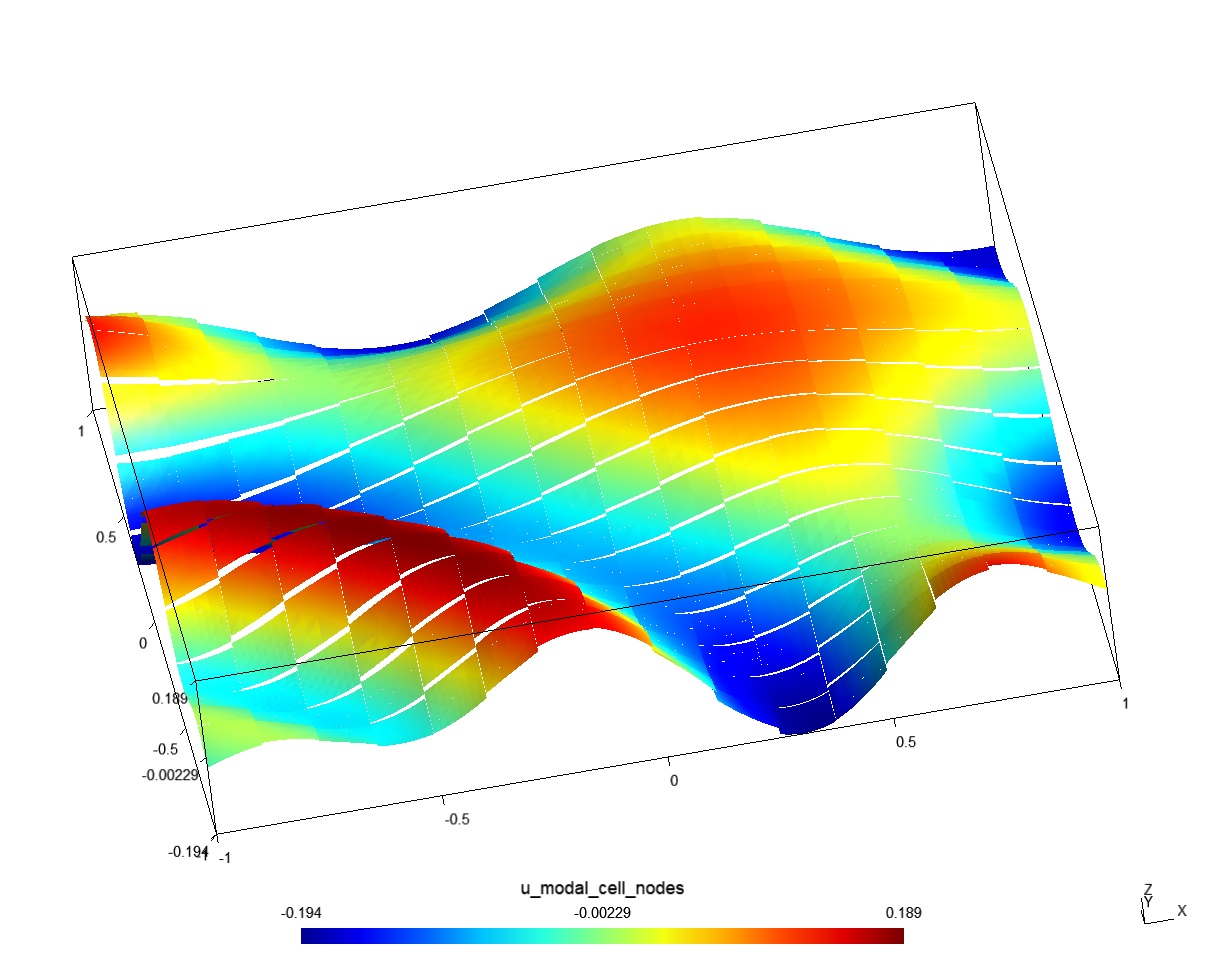
\includegraphics[width=\linewidth]{../figs/sols/kucera-010000000-sol-h256o02}
		\caption{$C_w = 1$}
	\end{subfigure}%
	\begin{subfigure}{.5\textwidth}
		\centering	
		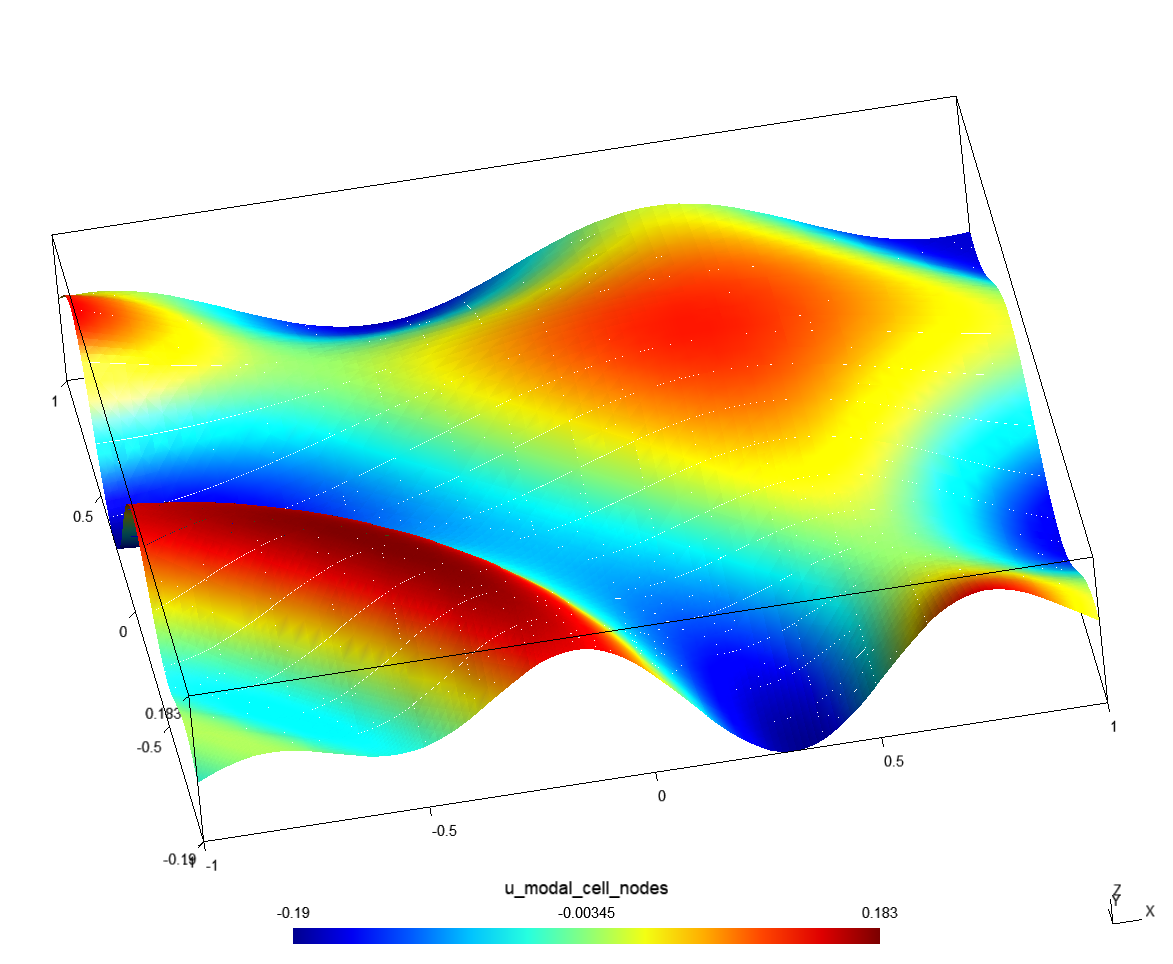
\includegraphics[width=\linewidth]{../figs/sols/kucera-212000000-sol-h256o02}
		\caption{$C_w = 15$}
	\end{subfigure}
	\caption{\Cref{ex:kucera}. Solution for different values of $C_w$ on a quadrilateral 
	mesh.}
	\label{fig:sol_kucera}
\end{figure}

\begin{figure}[p!]
	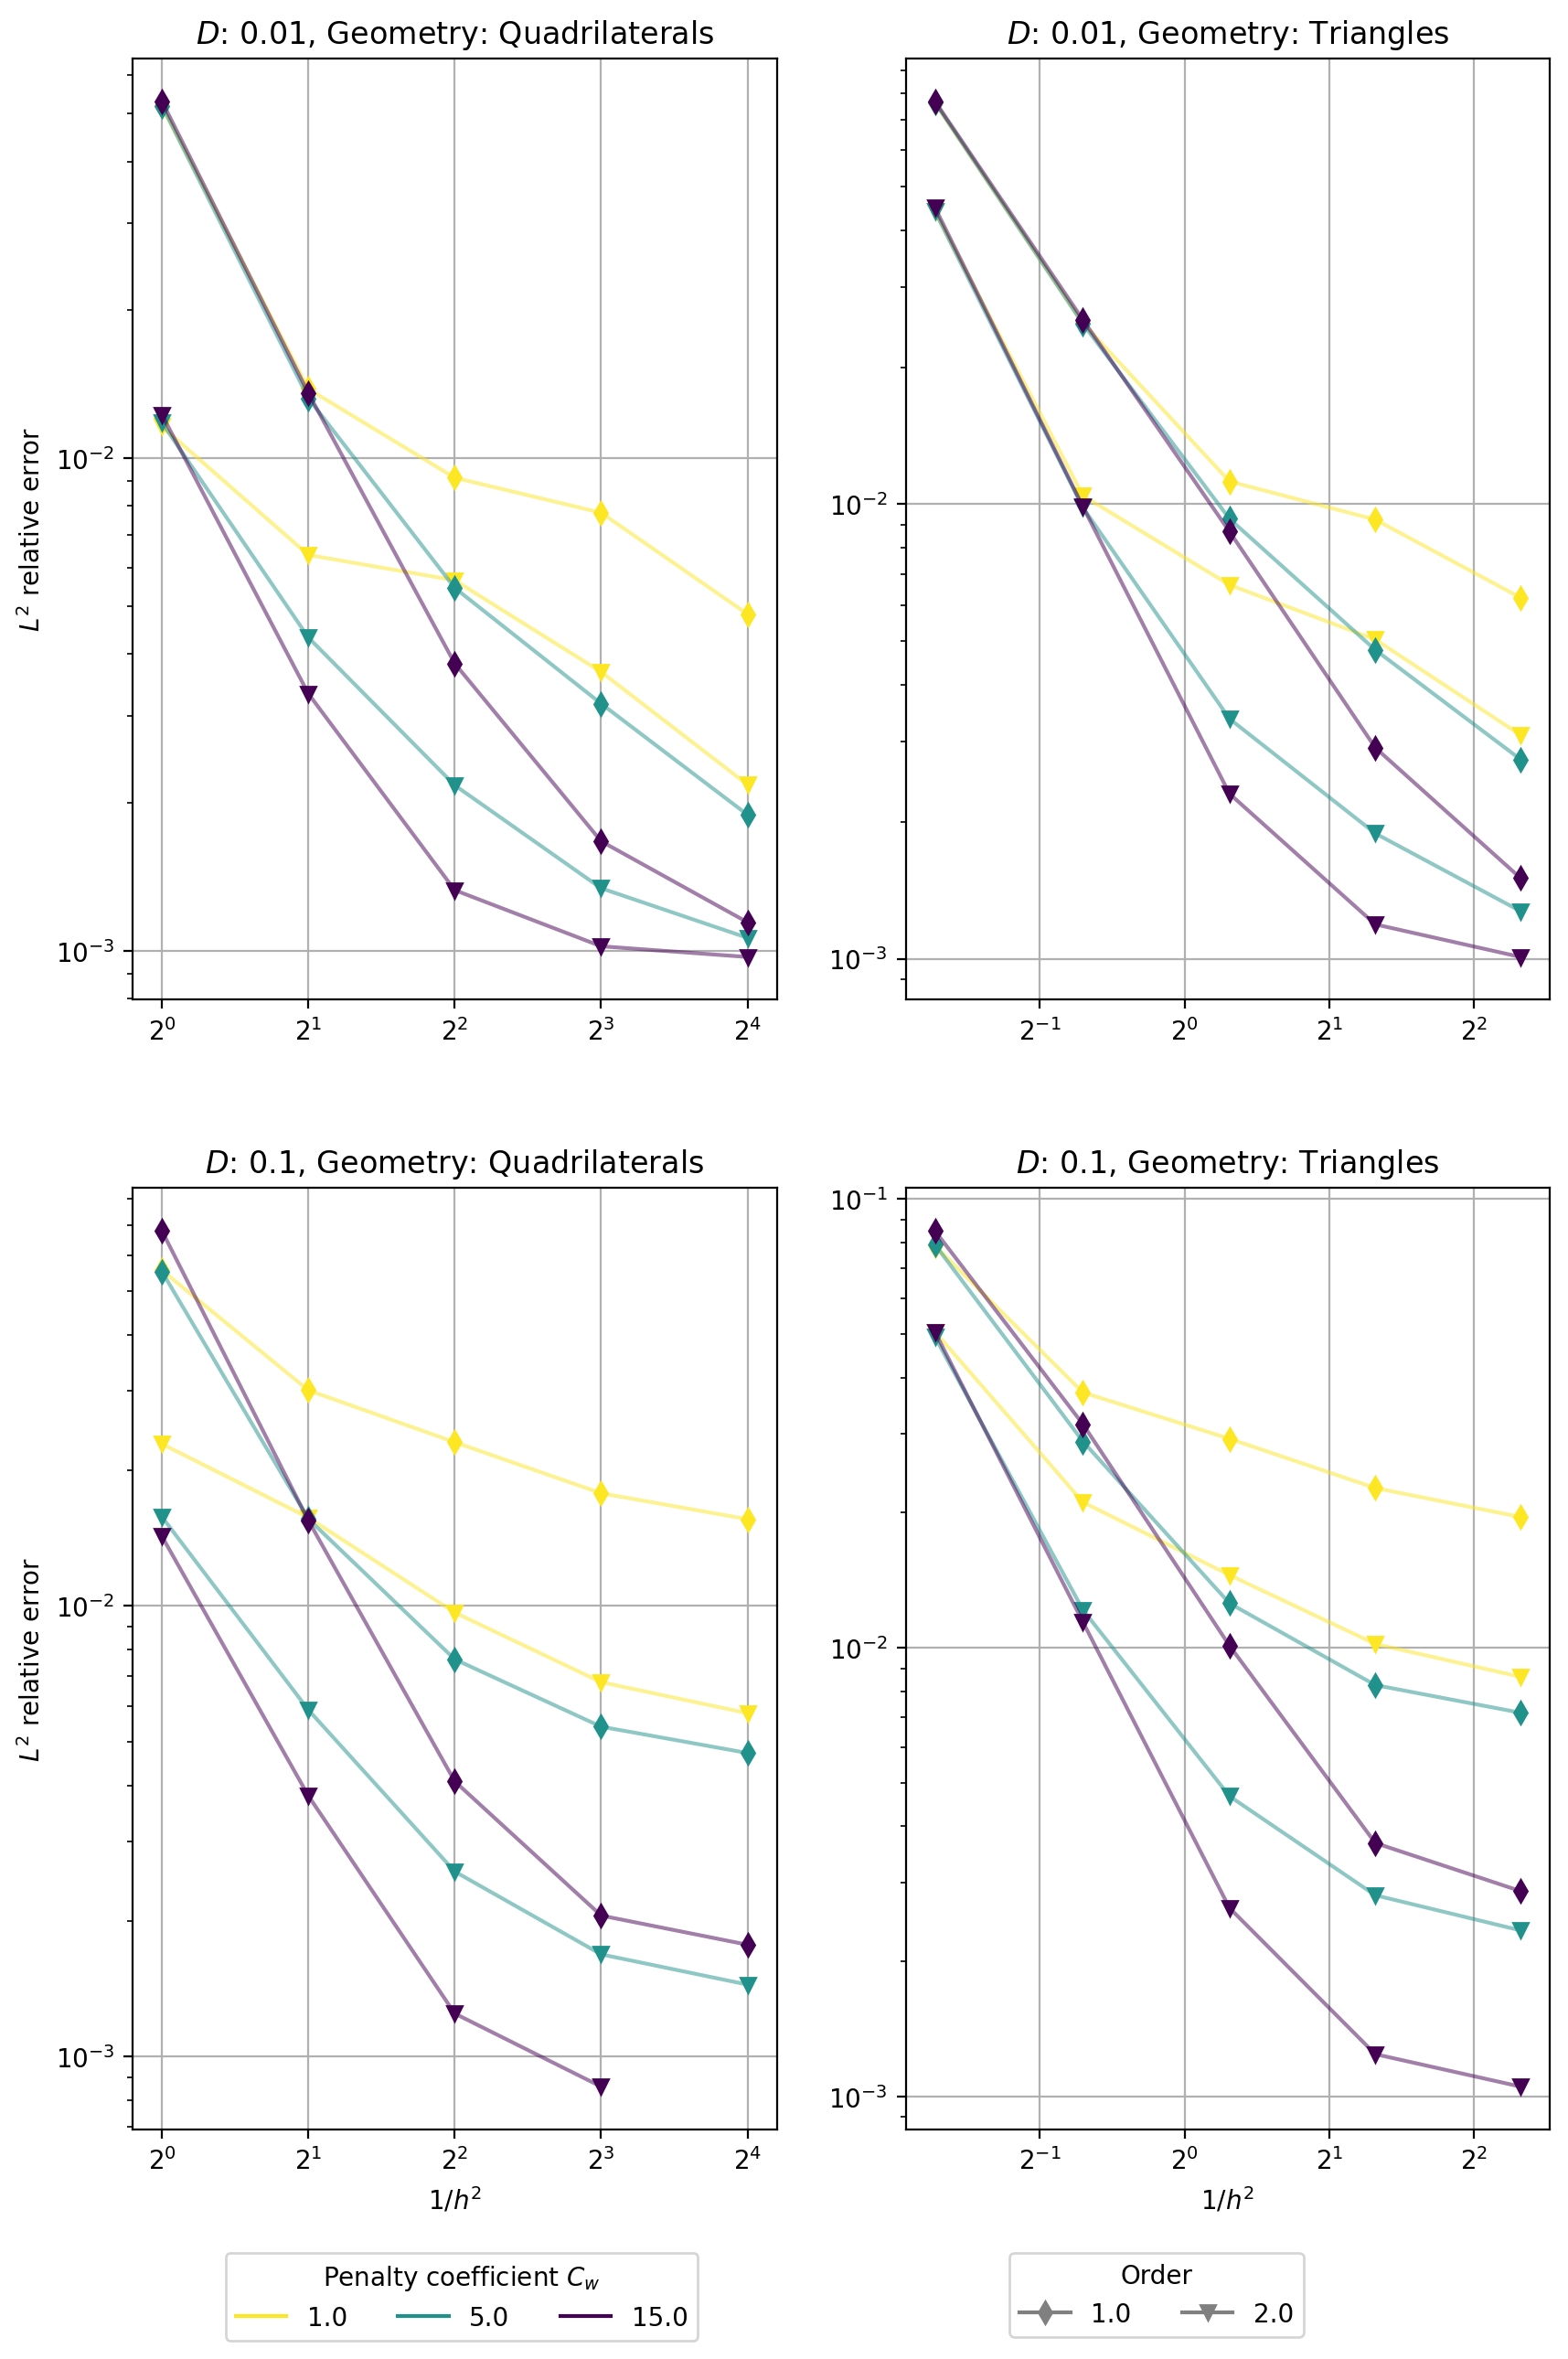
\includegraphics[width=\textwidth]{../figs/parametric/burgers_2D/convergence_symmetry}
	\caption{\Cref{ex:kucera}. Relative errors for different choices of $C_w$ for 
	quadrilaterals (left) and triangles (right).}
	\label{fig:kucera_conv}
\end{figure}
%\input{conv_burgess_hesthaven.tex}

\bibliographystyle{plain}
\bibliography{dg_fem_literature}
	
\end{document}